\documentclass[12pt,a4paper]{report}

%Set language
\usepackage[english]{babel}
\usepackage{enumerate}

% To import and adjust images
\usepackage{graphicx}
\usepackage[export]{adjustbox}
\usepackage[center]{caption}
\usepackage{subcaption}
\usepackage{float}
\usepackage{tabularx}

% To import alloy source code
\usepackage[dvipsnames]{xcolor}
\usepackage{listings}
\usepackage{alloy-style}

% Path relative to the .tex file containing the \includegraphics command
\graphicspath{ {./images/} }  

%To use enumerate

% To change the ToC title
\addto\captionsenglish{ \renewcommand {\contentsname} {Table of contents}}

\title{SafeStreets - RASD \\ \large version 1.0}
\author{Frangi Alberto, Fucci Tiziano}
\date{A.Y. 2019/2020}
\begin{document}
\maketitle

% Command to hide subsections in the index
\setcounter{tocdepth}{1}

% Index
\tableofcontents
\chapter{Introduction}
	\section{Purpose}
SafeStreets is a crowd-sourced application that intends to provide users with the possibility to notify authorities when traffic violations occur, and in particular parking violations, such as vehicles parked in the middle of bike lanes or in places reserved for people with disabilities, double parking, and so on. The application allows users to send pictures of violations, including their date, time, and position, to authorities.
 
SafeStreets stores the information provided by users, completing it with suitable meta-data. In particular, when it receives a picture, it runs an algorithm to read the license plate (one can also think of mechanisms with which the user can help with the recognition), and stores the retrieved information with theviolation, including also the type of the violation (input by the user) and the name of the street where the violation occurred (which can be retrieved from the geographical position of the violation). 

The application allows both end users and authorities to mine the information that has been received, for example by highlighting the streets (or the areas) with the highest frequency of violations, or the vehicles that commit the most violations. 

Moreover, if the municipality offers a service that allows users to retrieve the information about the accidents that occur on the territory of the municipality, SafeStrees can cross this information with its own data to identify potentially unsafe areas, and suggest possible interventions (e.g., add a barrier between the bike lane and the part of the road for motorized vehicles to prevent unsafe parking).


	\section{Scope}
	\subsection{General description}
Safestreet is an application to be used both from civilians (users) and authorities, in order to help the latter and reduce traffic violations. Registered authorities can automatically receive reports made by users, so the service acts as an intermediary. Reports are made of a picture of the violation and some... 
	%(to be reviewed and completed)
	\subsection{Goals}
	The following list describes the goals from the S2B perspective:
		\subsubsection{User}
	% Dot list 
	\begin{itemize}
		\item \textbf{G1}: The application must allow the users to register entering an e-mail address and a password.
		\item \textbf{G2}: The application must allow the users to notify traffic violations, providing  the type of violation and a picture of the vehicle.
	% Il resto se lo trova da solo
		\item \textbf{G3}: The application must be able to show to the users the streets and the vehicles with the highest frequency of violations.
		\item \textbf{G4}: The application must allow the user to see all of his reports and their status.
		\item \textbf{G5}: The application must notify the user when one of his reports is evaluated.
	\end{itemize}
		\subsubsection{Authority}
	\begin{itemize}
		\item \textbf{G6}: The application must allow the authorities to register providing a valid identification number and a valid password.
	  	\item \textbf{G7}: The application must allow authorities to retrieve and evaluate the available reports.
		\item \textbf{G8}: The application must be able to identify potentially unsafe areas and suggest possible interventions.
	\end{itemize}
	

	\section{Definitions, acronyms, abbreviations}
		\subsection{Definitions}
		\begin{itemize}
		\item \textbf{User}: a civilian customer that can use the application to:
			\begin{itemize}
			\item notify authorities of some violation;
			\item check which are the most dangerous (i.e. with the most violations) streets;
			\item check which are the vehicles that committed the most violations.
			\end{itemize}
		\item \textbf{Authority}: a member of the local police who has access to reports made by users.
		\item \textbf{Report}: a message consisting of:
			\begin{itemize}
			\item a picture showing the car in order to show the occurring violation;
			\item date and time of the picture;
			\item GPS position of the place where the violation occurred;
			\item the street where the violation occurred (automatically retrieved from the geographical position);
			\item the type of the violation (input by the user)
			\end{itemize}
		\item \textbf{Available}: a report is available for an authority if its position is within the municipality assigned to the authority.
		\item \textbf{Violation}: a situation that, according to the user who sent the report, is a violation of the traffic laws.
		\item \textbf{Intervention}: a brief text suggesting a possible solution in order to improve safety and discourage future violations.
		\end{itemize}
		\subsection{Acronyms}
			\begin{itemize}
			\item \textbf{API}: \emph{Application Programming Interface.}
			\item \textbf{GPS}: \emph{Global Positioning System.}
			\item \textbf{UI}: \emph{User Interface.}		
			\item \textbf{S2B}: \emph{Software-to-be.}	
			\end{itemize}
		\subsection{Abbreviations}
% To be written

	\section{Revision history}
% To be written

	\section{Reference documents}
	\begin{itemize}
	\item {Specification document}: ``SafeStreets Mandatory Project Assignment''
	%to be completed
	\end{itemize}

	\section{Document structure}
	\begin{itemize}
	\item \textbf{Chapter 1} is an introduction: it presents the document and the S2B with its scope and goals. It also helps the reader to understand, by giving the necessary definitions and explaining acronyms and abbreviations. 
	\item \textbf{Chapter 2} is a summary description of all the project and how the main parts work. %Non so, ti va bene? i
	\item \textbf{Chapter 3} is the core of the document...
	\item \textbf{Chapter 4} contains the Alloy model of critical aspects that require special attention. Here it is shown how the project has been modeled and a proof of the model consistency is provided. Moreover, examples of some of the generated world are shown.
	\item \textbf{Chapter 5} is meant to show how work was divided between the two components of the group and how much time was spent.
	\item \textbf{Chapter 6} contains the list of references...
	\end{itemize}

% End of first chapter

\chapter{Overall description}
	\section{Product perspective}
		Safe Streets want to be a mediator between authorities and citizen, allowing the last ones to report traffic violations, see
		in which zone have the highest number of violations, and the recap of all the previous reports and their state
		(seen, approved, rejected, in queue). In order to be able to report various violations an user has to be in first place in a
		territory covered by any authorities who had signed up to Safe Streets, and has to sign up compiling a form, choosing a
		nickname, unique for each user, and a mail. Any authority has to verify its identity using the institutional email 
		The system to avoid spamming of request pending reports will be in a priority queue based 
		on a reliability index associated to each user and hidden to both side of communication (is an information used only by 
		the system for the priority queue). If the authorities sanction a violation reported the user 
		will receive a notification by Safe Streets to inform him the success (or failure) of his report. 
		\begin{figure}[H]
			\begin{subfigure}{\textwidth}
				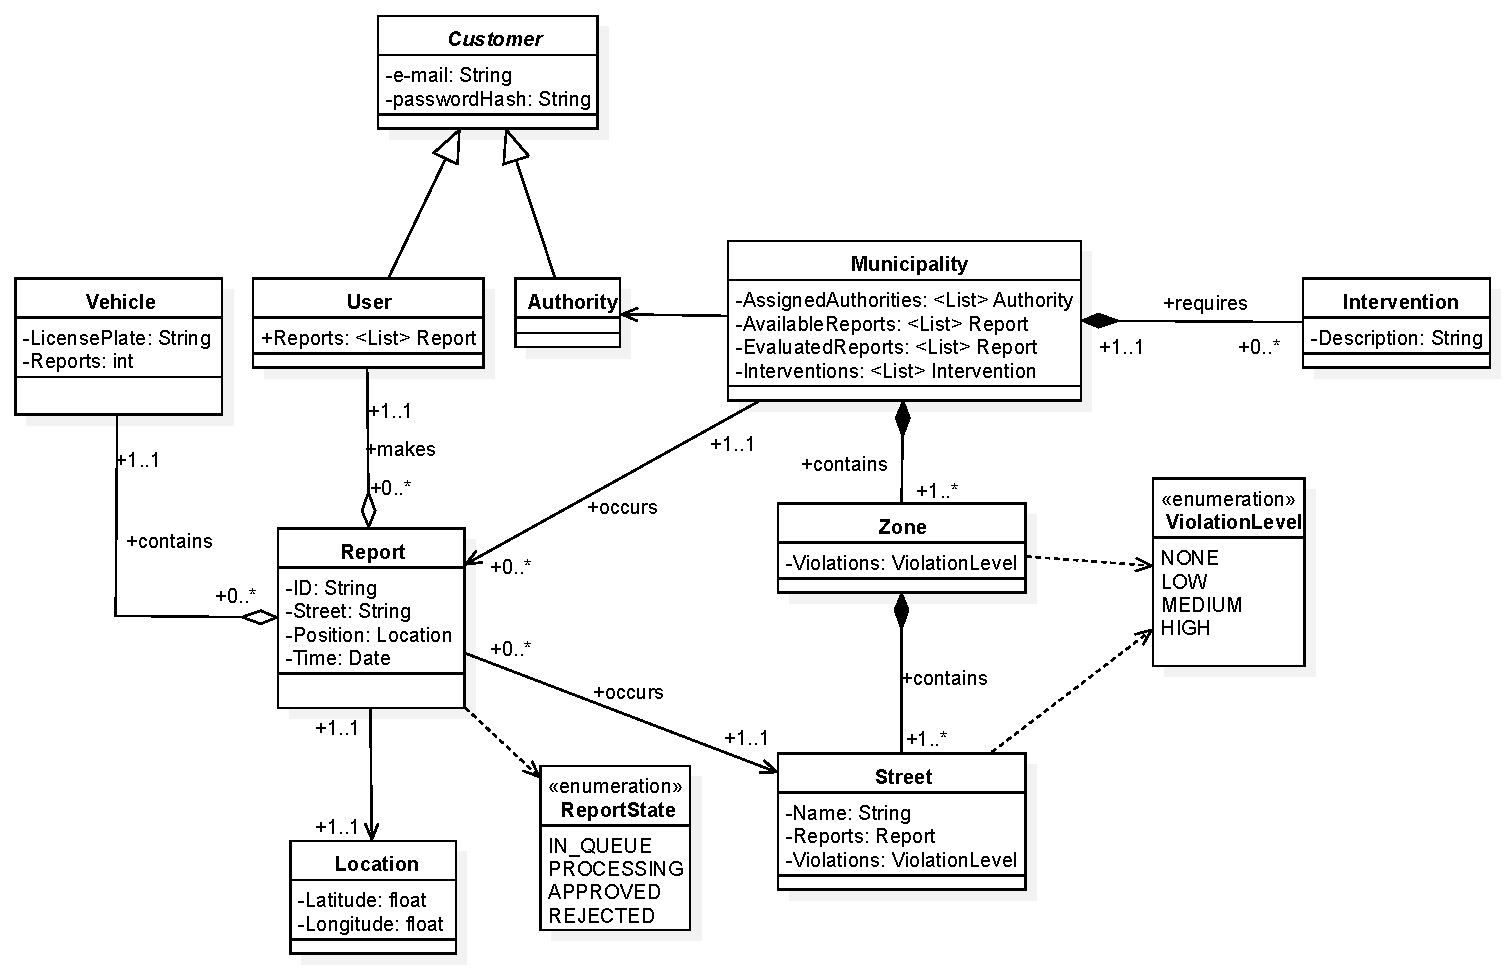
\includegraphics[scale = 0.75, center]{uml}
				\caption{UML model}
				\label{UML model }
			\end{subfigure}
		\end{figure}
		This figure represent a draft of how the system's UML model is supposed to look like. Because it is only the model part the 
		classes represented are only the few essential to save correctly all the data necessary for all the analysis and to be displayed
		(respectively that are part of controller and view) and in order to save up space we avoided to write every single getter and setter.
		A generic Customer has been model with an abstract class and both authorities and User inherit it.
		Report is a combination of various classes, it contains an unique id, the Street (obtained by the gps position), the time (obtained
		by the system when it receive the report), the vehicle license's plate and the type of violation, it has also an enum attribute
		to represent the status of the report. Both ``Street" and ``Zone" (which is a group of streets) contains a ViolationLevel, that
		is calculated by the system and based on the reports' number in that particular street/zone. Intervention is a suggestion made
		by the system on municipality's request, is created by a recommender system that apply some simple data mining's algorithm
		in order to find the best improvement for each street based on the most frequent violations or accidents.
		Municipality contains a list of possible interventions, all the authorities that operates in its territory and all reports
		(both evaluated and to evaluate).

		
		Now we are going to analyze some critical aspects of the application, modeling their behaviors and	
		showing the evolution over time of their	states	through appropriate state diagrams, which are
		reported below.
		
		\begin{figure}[H]
			\begin{subfigure}{\textwidth}
				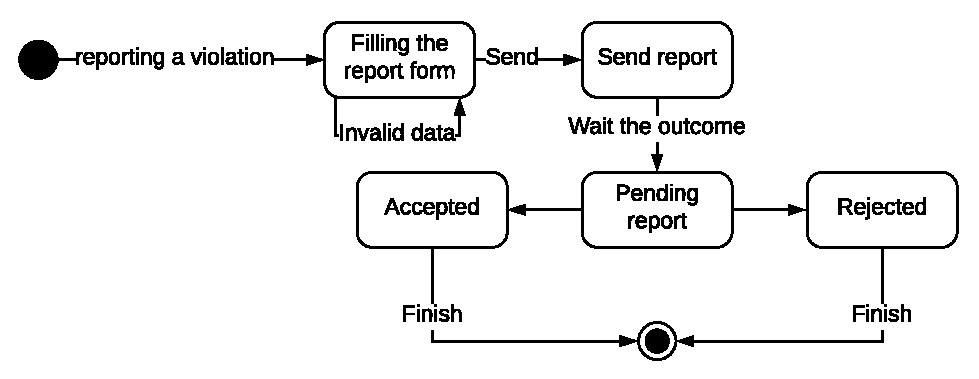
\includegraphics[scale = 0.75, center]{reportC}
				\caption{State diagram on the behavior of reports for citizen}
			\end{subfigure}
		\end{figure}
		This diagrams represent the behavior of the reporting system (for the citizen), is pretty straight forward. The system doesn't allow report
		with missing information or with wrong ones.
		
		\begin{figure}[H]
			\begin{subfigure}{\textwidth}
				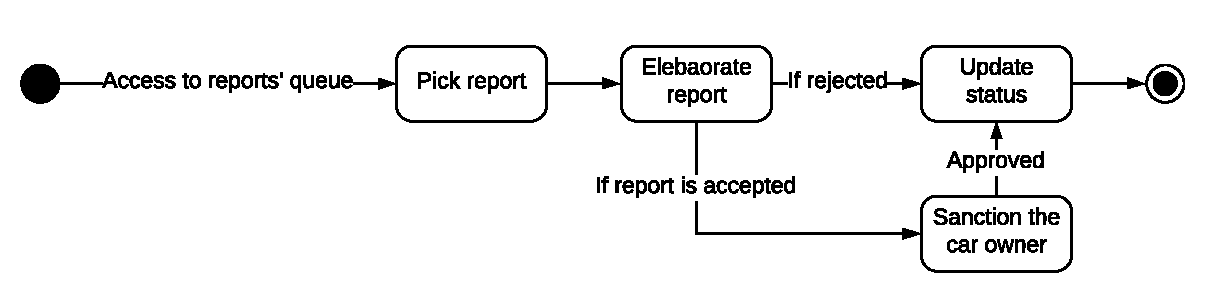
\includegraphics[scale = 0.75, center]{reportA}
				\caption{State diagram on how reports work for authorities}
			\end{subfigure}
		\end{figure}	
		This diagram is inherent to the reports verification process,
		it show the evolution of the states necessary to handle a report, from when the authorities take in charge an user's report
		to the eventual sanction to the car owner.
		
		\begin{figure}[H]
			\begin{subfigure}{\textwidth}
				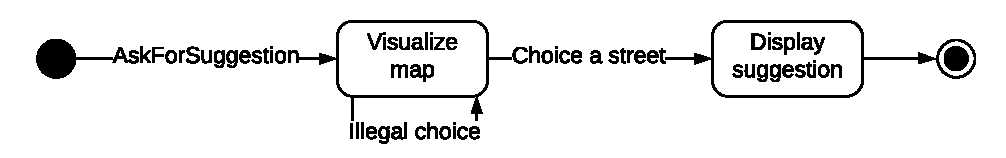
\includegraphics[scale = 0.75, center]{suggestion}
				\caption{State diagram on how reports work for authorities}
			\end{subfigure}
		\end{figure}
		This last diagram represent how the last major functionality offered by SafeStreet. It consist in a system that offers suggestion
		on how improve the safety on particular streets, based on the occurrence of car accident and street violations data that
		the authorities choose to share with SafeStreets.
		  
		
	\section{Product functions}
		In the following section the most important product functions of the system are reported.
		Safe Streets offers the possibility to its users to report traffic violations, check the status of the previous reports and see 
		a map that indicates the areas with the highest number of report verified.
		\subsection{Report}
			To report a violation a user has to take a picture of the possible violation with the plate visible, choose what type of
			violation it is from various possible categories and send the position.
		\subsection{Status}
			This functionality allows user to see a recap of all the reports they have made. The information that will be displayed
			are: Date and time, place, type of violation and status. The last one can be:
			\begin{itemize}
				\item \textbf{In queue:}
					In this status the report is waiting to be analyzed by an authority. The report's priority is based on
					the user who created it. All the user at the moment of registration has a standard value that based on
					how Safe Street is used can increase or decrease. Some important factors are, for example, 
					how many report a user sent has been rejected, how many report a user send in one time can decrease
					the priority, but a wisely use of the system can increase it, like a streak of approved reports.
				\item \textbf{Processing:}
					In this status the authorities has seen the report and are considering the violation and if it is a real
					violation.
				\item \textbf{Approved:}
					The report has been seen by authorities and the violation has been recognized and sanctioned 
				\item \textbf{Rejected:}
					The report has been seen by authorities and the violation hasn't been recognized.
			\end{itemize}
		\subsection{Map}
			This function allows the user to open the map and see the "level of violations" of the different areas. These "levels" are
			based on how many reports have been approved in that area, higher the level, higher the number of violation.
			There are 4 levels, are indicated with different color, from no colour (level 0) to red (level 3).
			
	\section{User characteristics}
		The actors of the application are the following:
		\begin{itemize}
			\item \textbf{User:}
				a person who has registered to SafeStreets, he doesn't need any particular skill to use the system, 
				he is just supposed to have a smartphone (or tablet) with a functioning camera, an internet connection and
				that his phone can send his current position. The user can send a report to notify the authorities various traffic
				violation, he can view a map that highlight the streets with an higher number of reports. To do a report is sufficient
				take a photo of the license plate, the violation's type and the system retrieves in autonomous the current position
				of the user.
			\item \textbf{Authority:}
				An agent of the local police of a municipality using SafeStreets, that has access to all the reports made
				 in his municipality. The authority can visualize the available reports and valuate them, that is telling if the
				violation reported by the user stands or it is not a proper violation. After seeing a report, the authority 
				changes its status to Approved or Rejected and if they activated
				an optional service they can check the streets with the highest number of accident and receive
				a suggestion (made by the system) about improve the safety.
		\end{itemize}
	\section{Assumptions, dependencies and constraints}
	\subsection{Domain assumption}
% Forse ce ne vuole qualcuna in più?
Maybe trivial assumptions can be omitted?
		\begin{itemize}
			\item \textbf{D1}: The users always provide a picture that allows both the algorithm to read the license plate and
					        the authority to identify the violation.
			\item \textbf{D2}: Every user is provided with a device capable to share the exact GPS position at any moment.
			\item \textbf{D3}: The name of the street where a violation occured is retrieved from the GPS position.
			\item \textbf{D4}: Authorities never make mistakes in evaluating a report.
			\item \textbf{D5}: Reports are evaluated only one time.
			\item \textbf{D6}: The user sends the report staying in the same place of the violation. attached to reports.
			\item \textbf{D7}: The picture of the license plate is taken at the moment and shows the right car.
		\end{itemize}


% End of second chapter

\chapter{Specific Requirments}
	\section{External interface requirments}
		\subsection{User interfaces}
		In this section some screenshots from the user interface are shown. Figures from (g) to (j) 
		\begin{figure}[H]
		\begin{subfigure}{0.5\textwidth}
			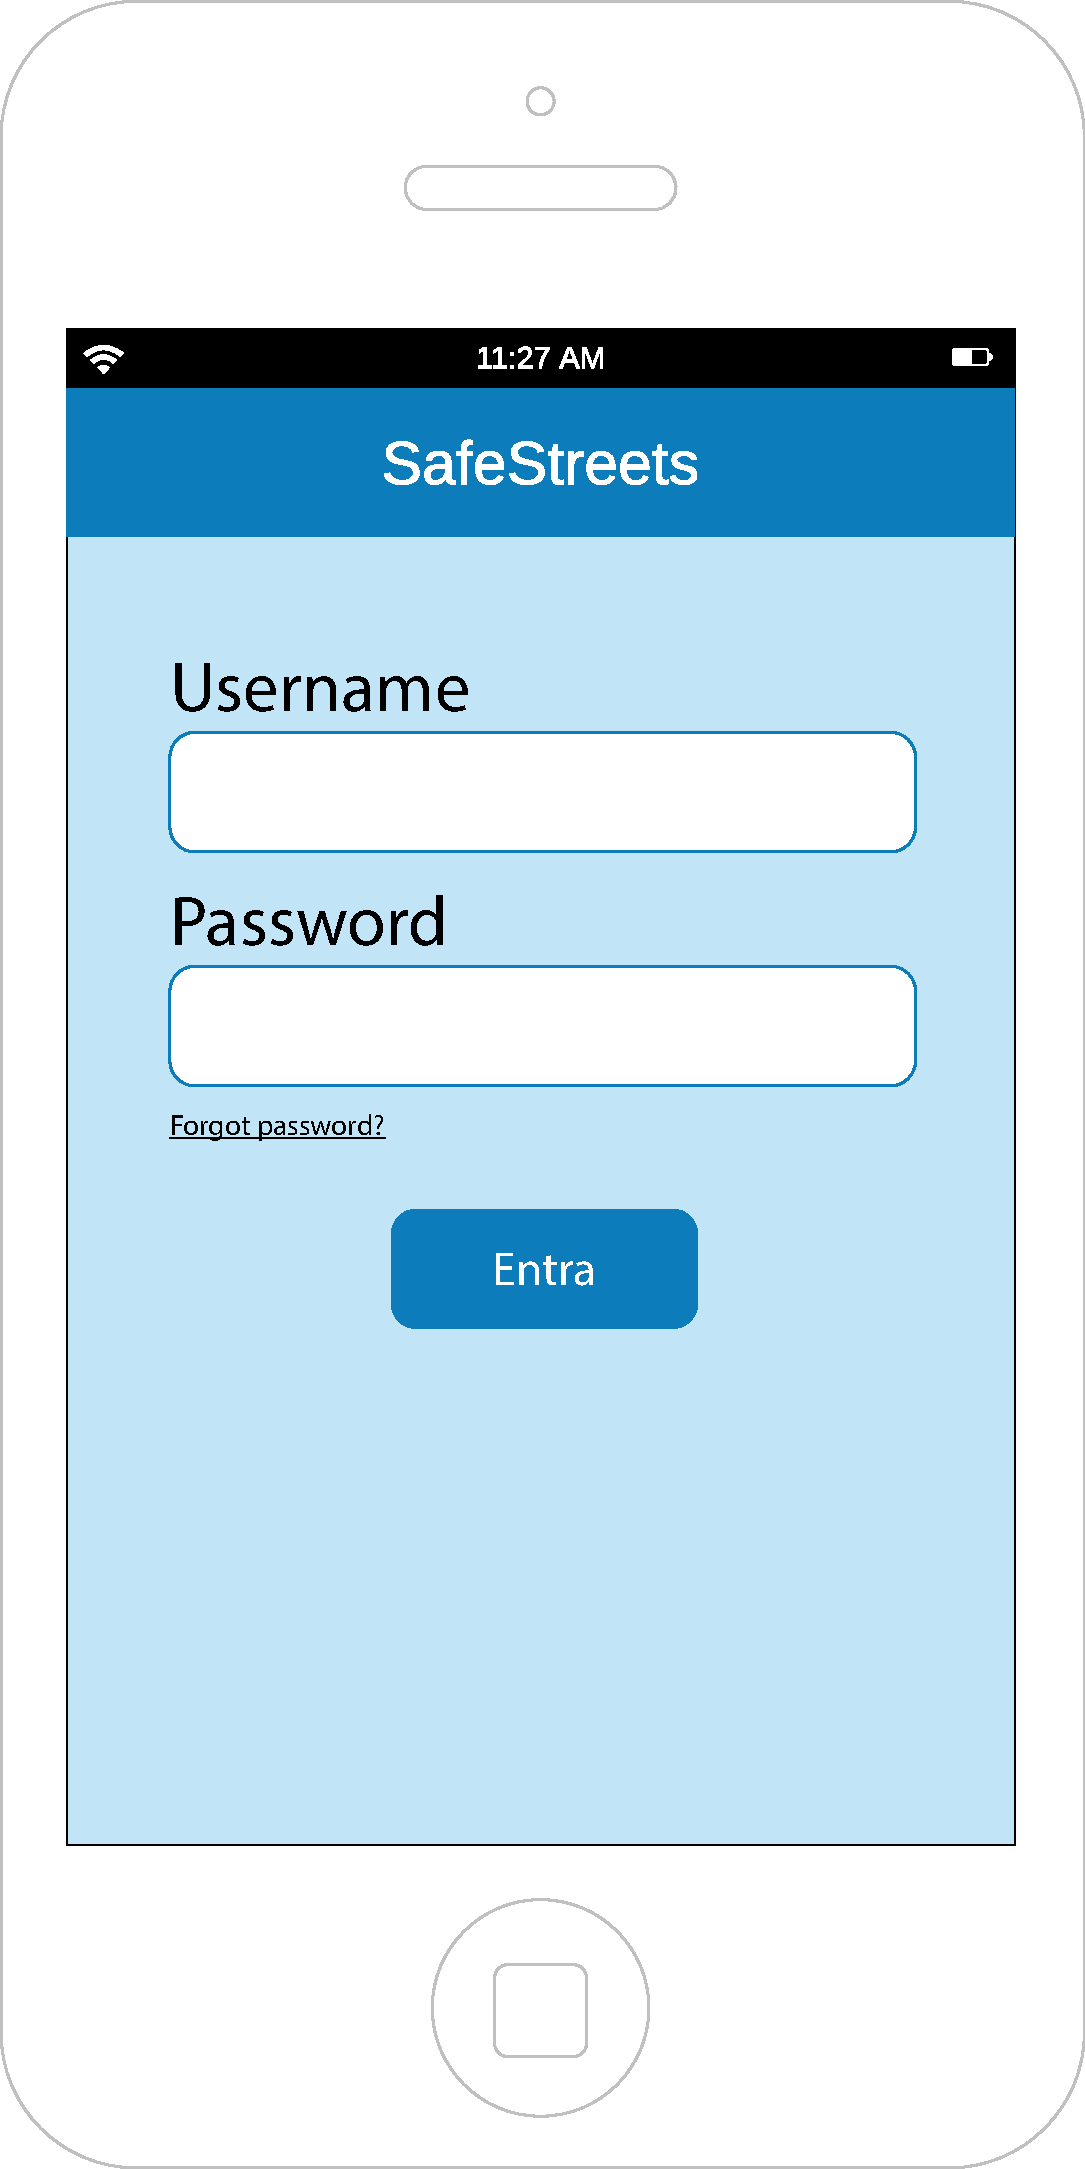
\includegraphics[scale=0.25, center]{Login}
			\caption{User - login}
			\label{Login}
		\end{subfigure}
		\begin{subfigure}{0.5\textwidth}
			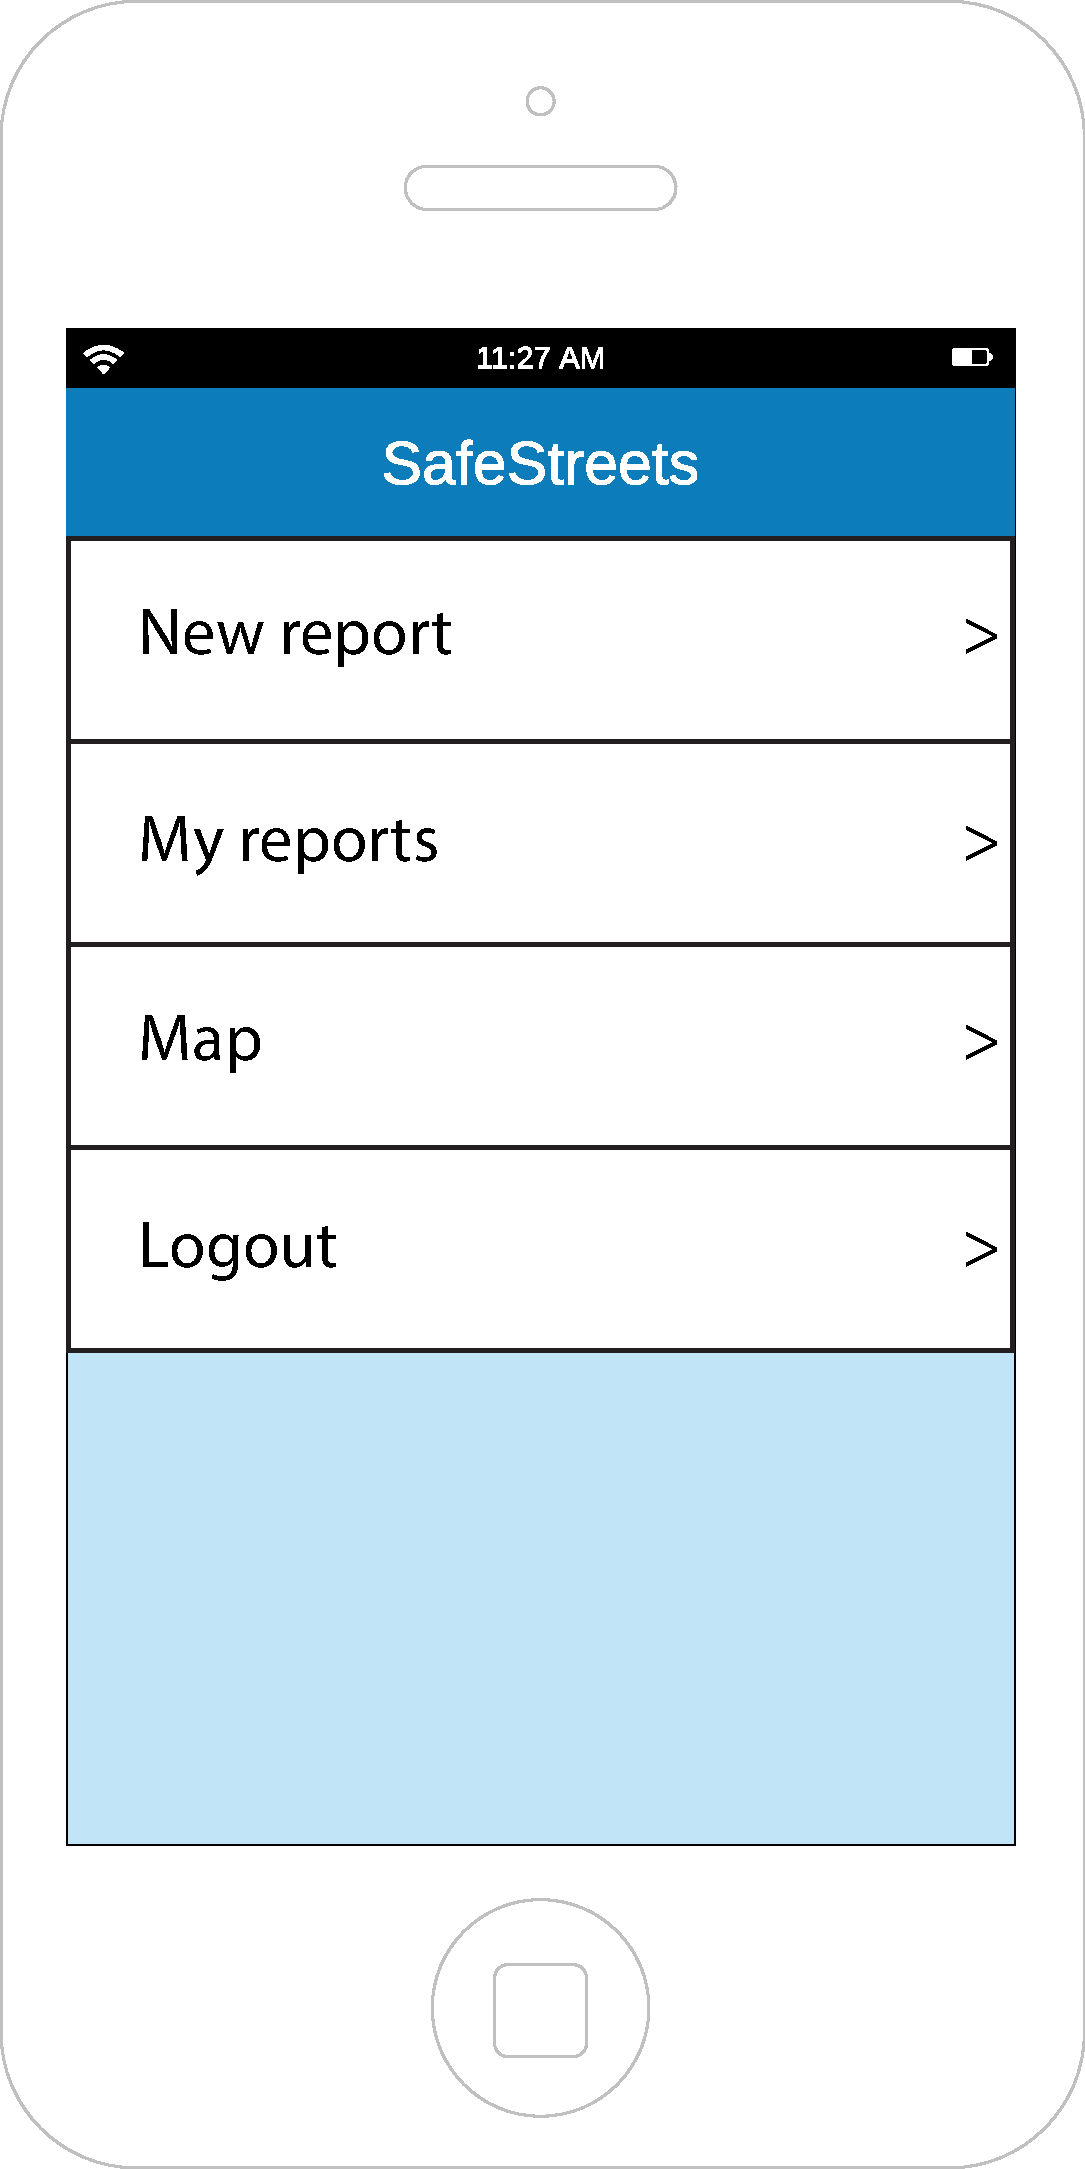
\includegraphics[scale=0.25, center]{Home}
			\caption{User - home}
			\label{Home}
		\end{subfigure}
		\end{figure}

		\begin{figure}[H]
		\begin{subfigure}{0.5\textwidth}
		\setcounter{subfigure}{2}
			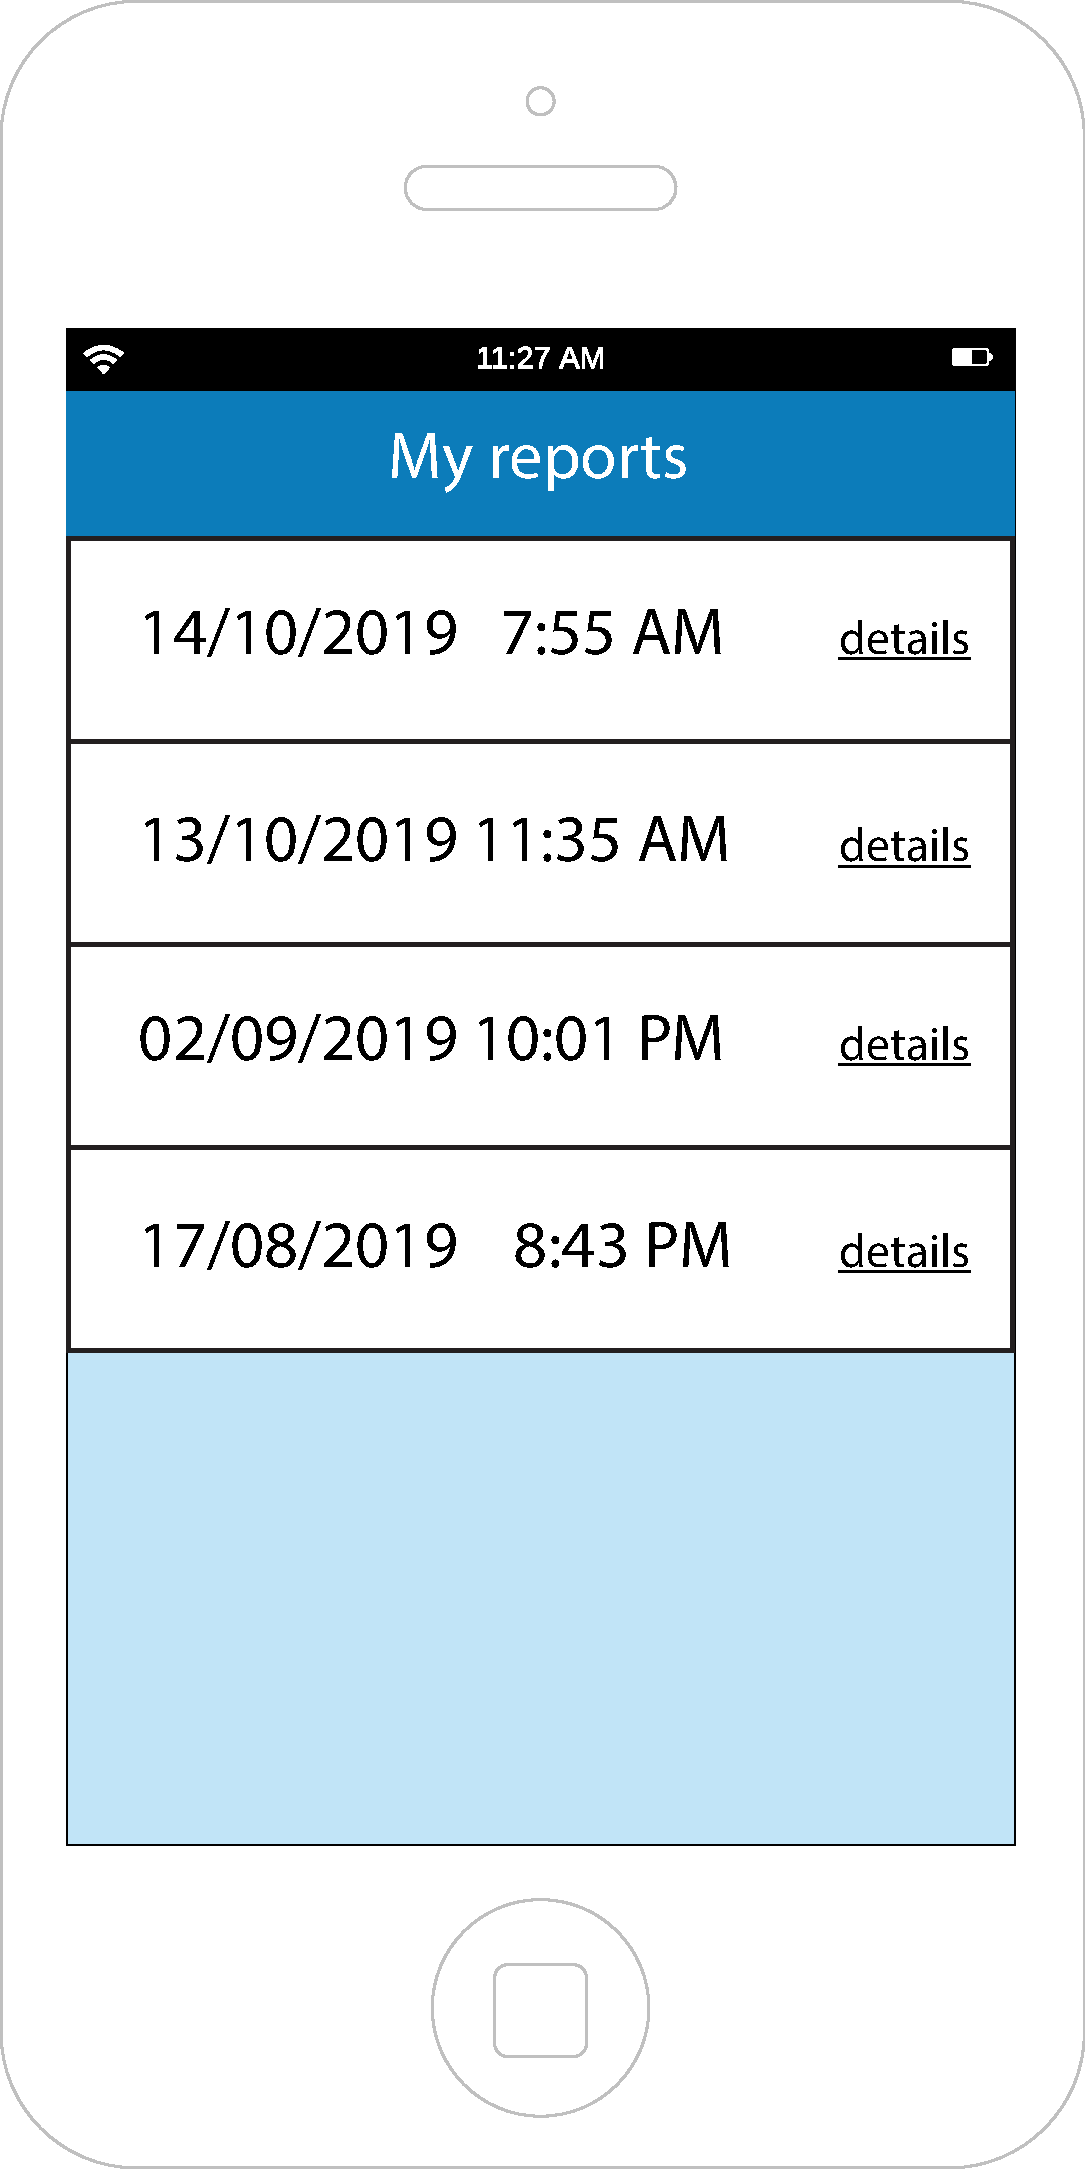
\includegraphics[scale=0.25, center]{Myreports}
			\caption{User -  list of sent reports}
			\label{List of sent reports}
		\end{subfigure}
		\begin{subfigure}{0.5\textwidth}
			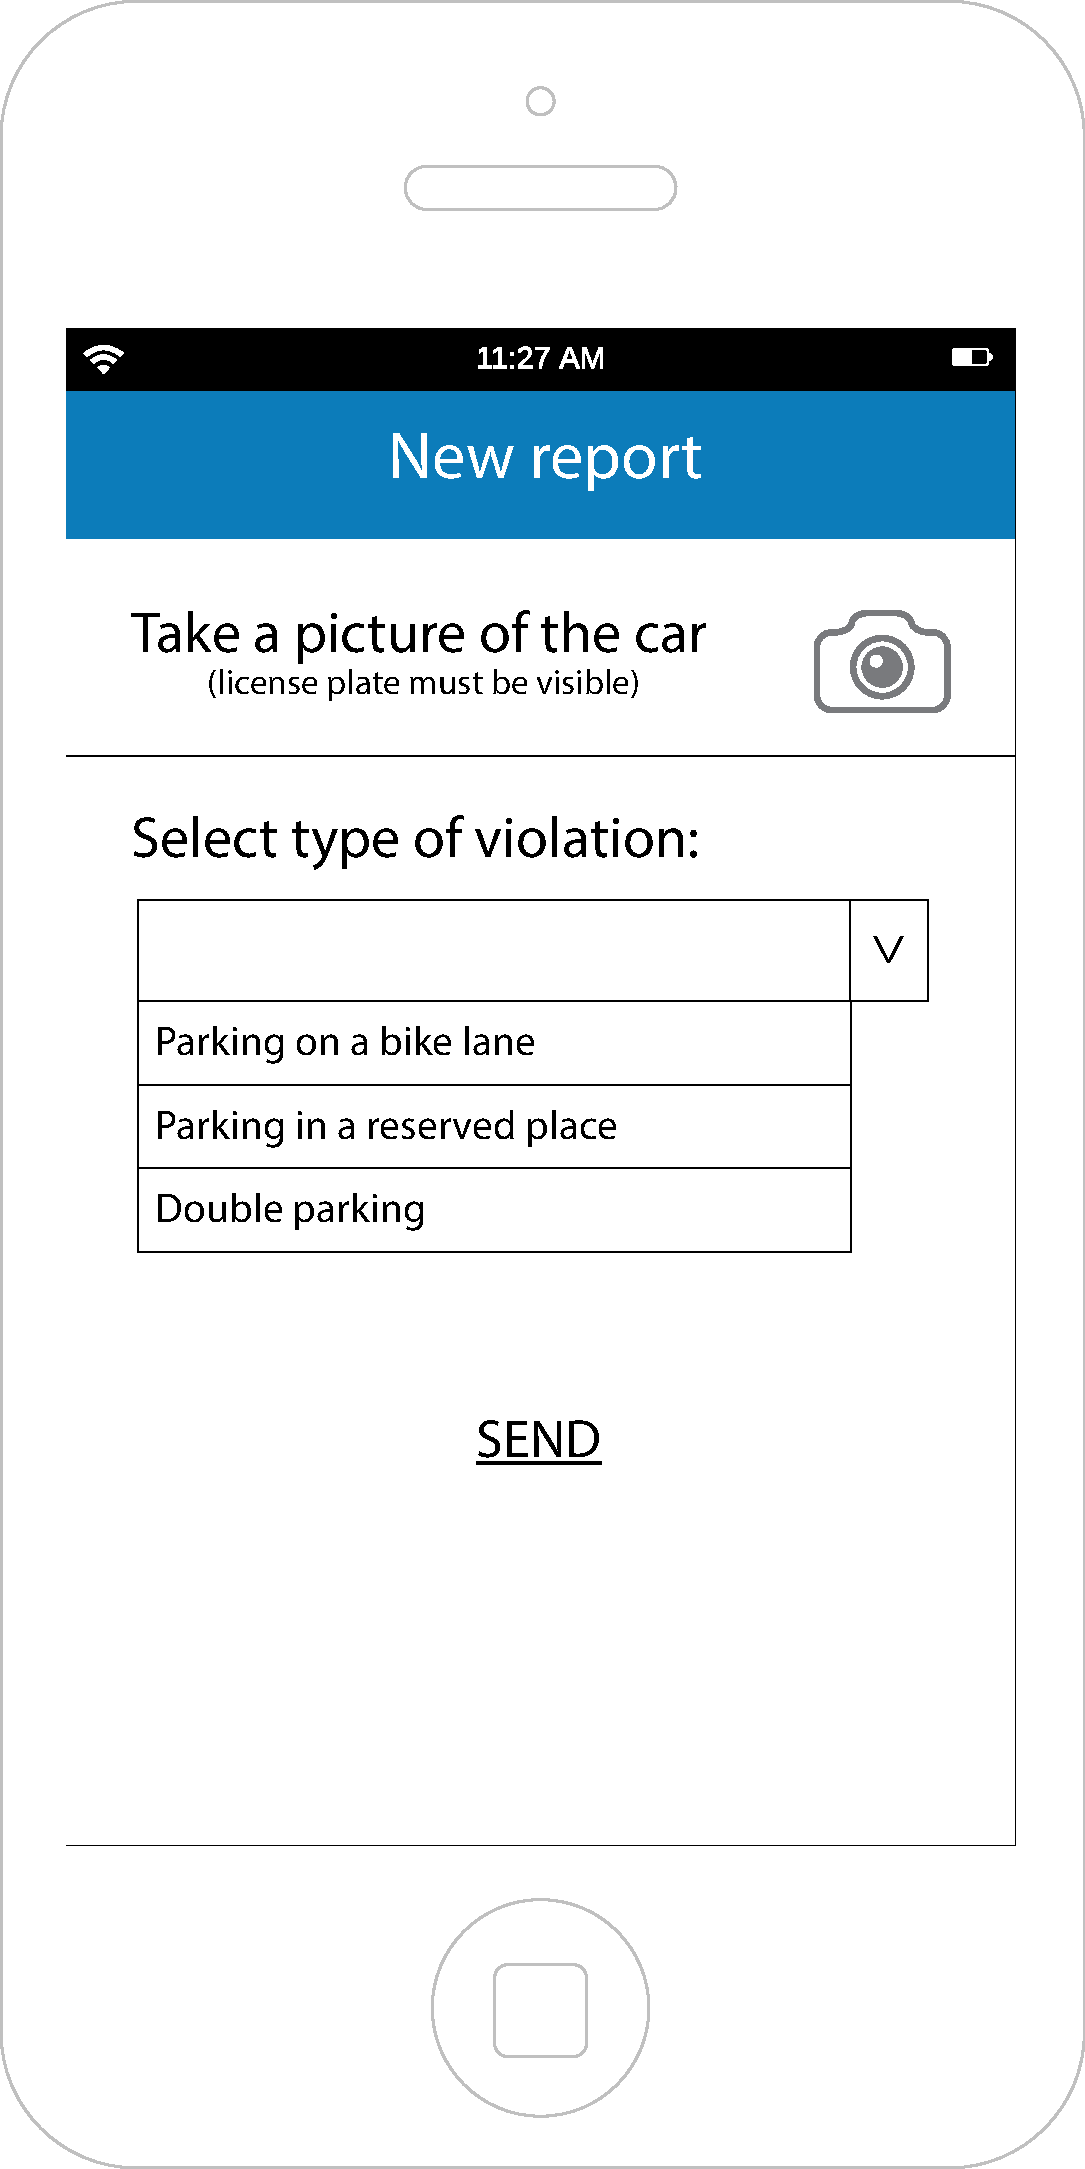
\includegraphics[scale=0.25, center]{Newreport}
			\caption{User -  new report}
			\label{fig:subim2}
		\end{subfigure}
		\end{figure}

		\begin{figure}[H]
		\begin{subfigure}{0.5\textwidth}
		\setcounter{subfigure}{4}
			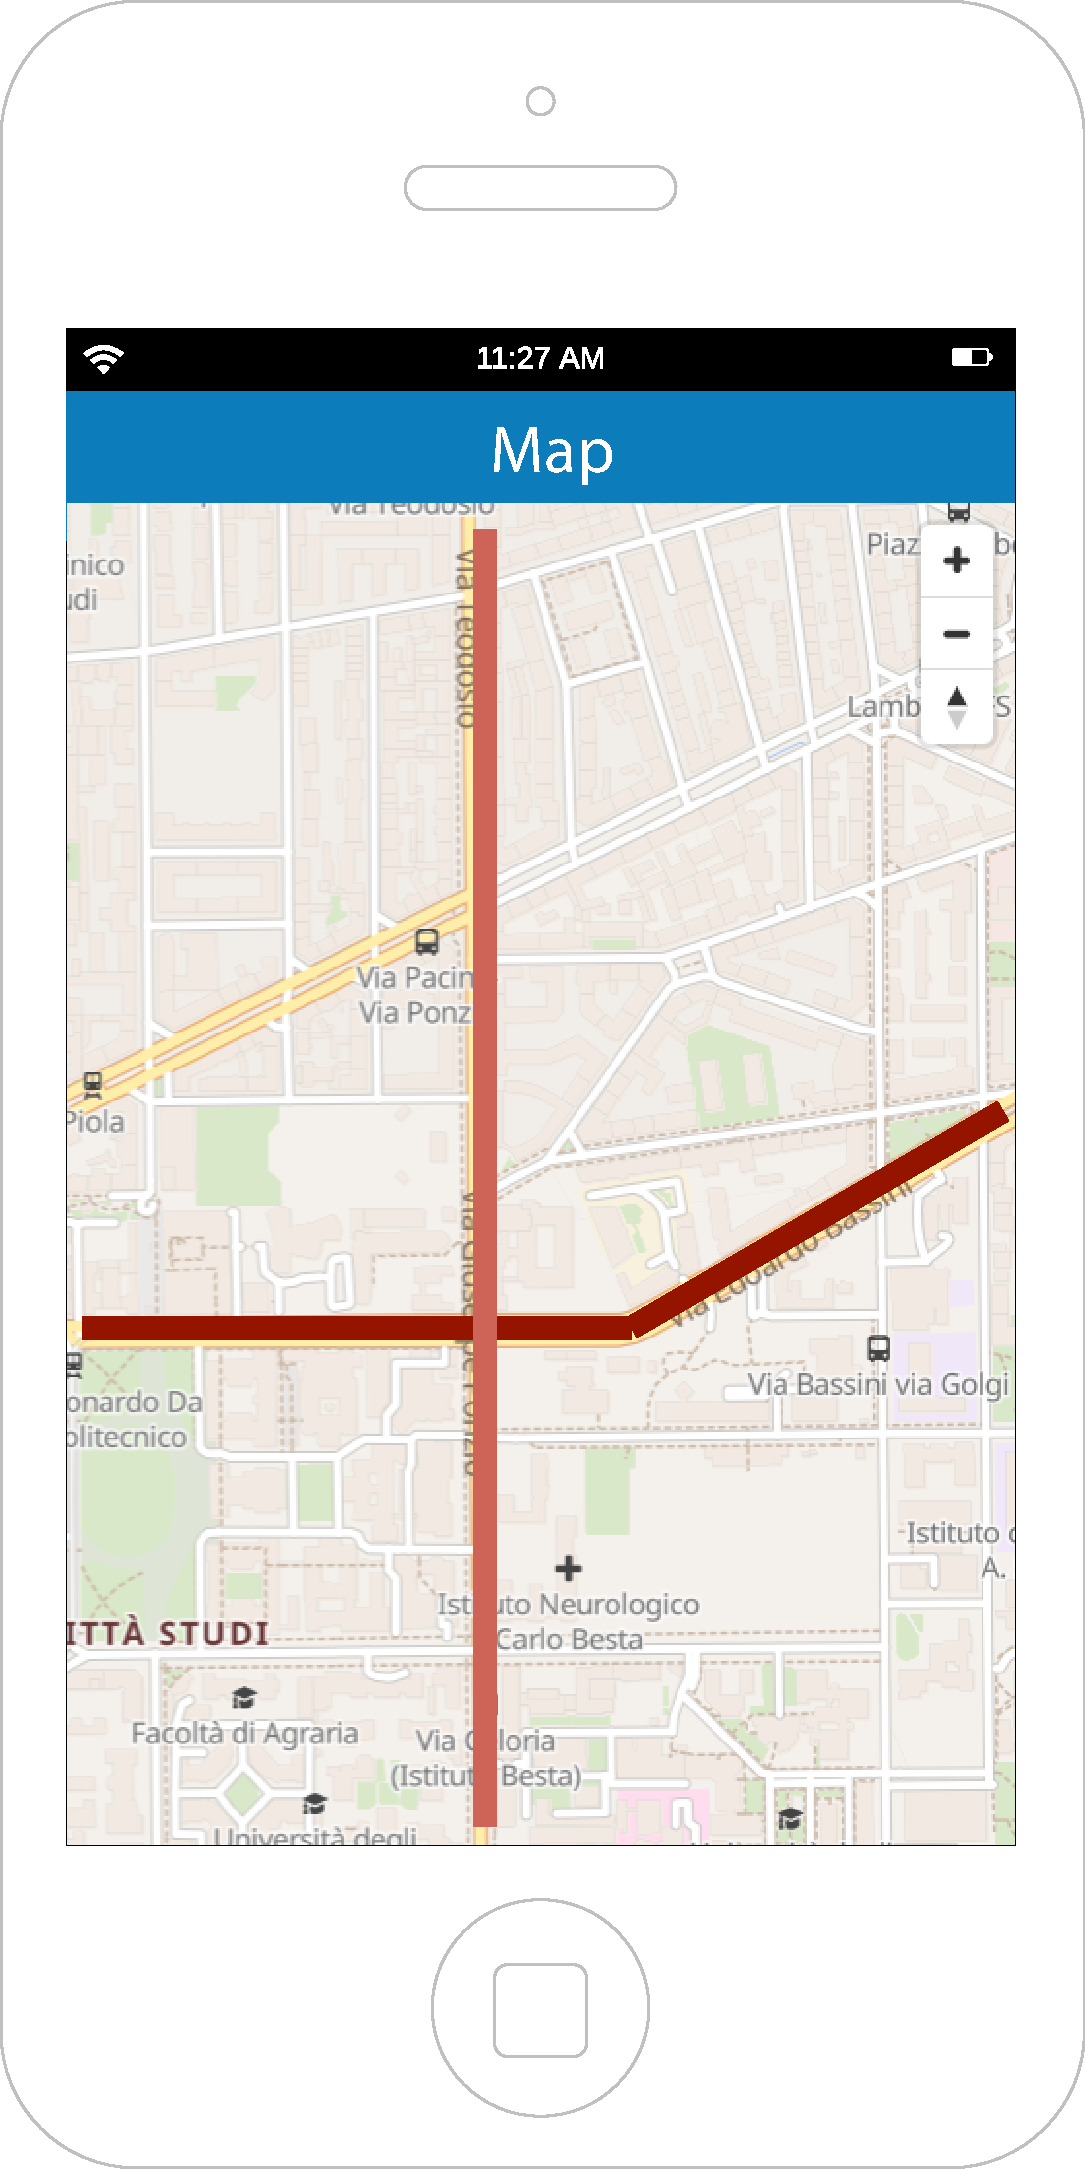
\includegraphics[scale=0.25, center]{Map}
			\caption{User -  map}
			\label{fig:subim2}
		\end{subfigure}
		\begin{subfigure}{0.5\textwidth}
			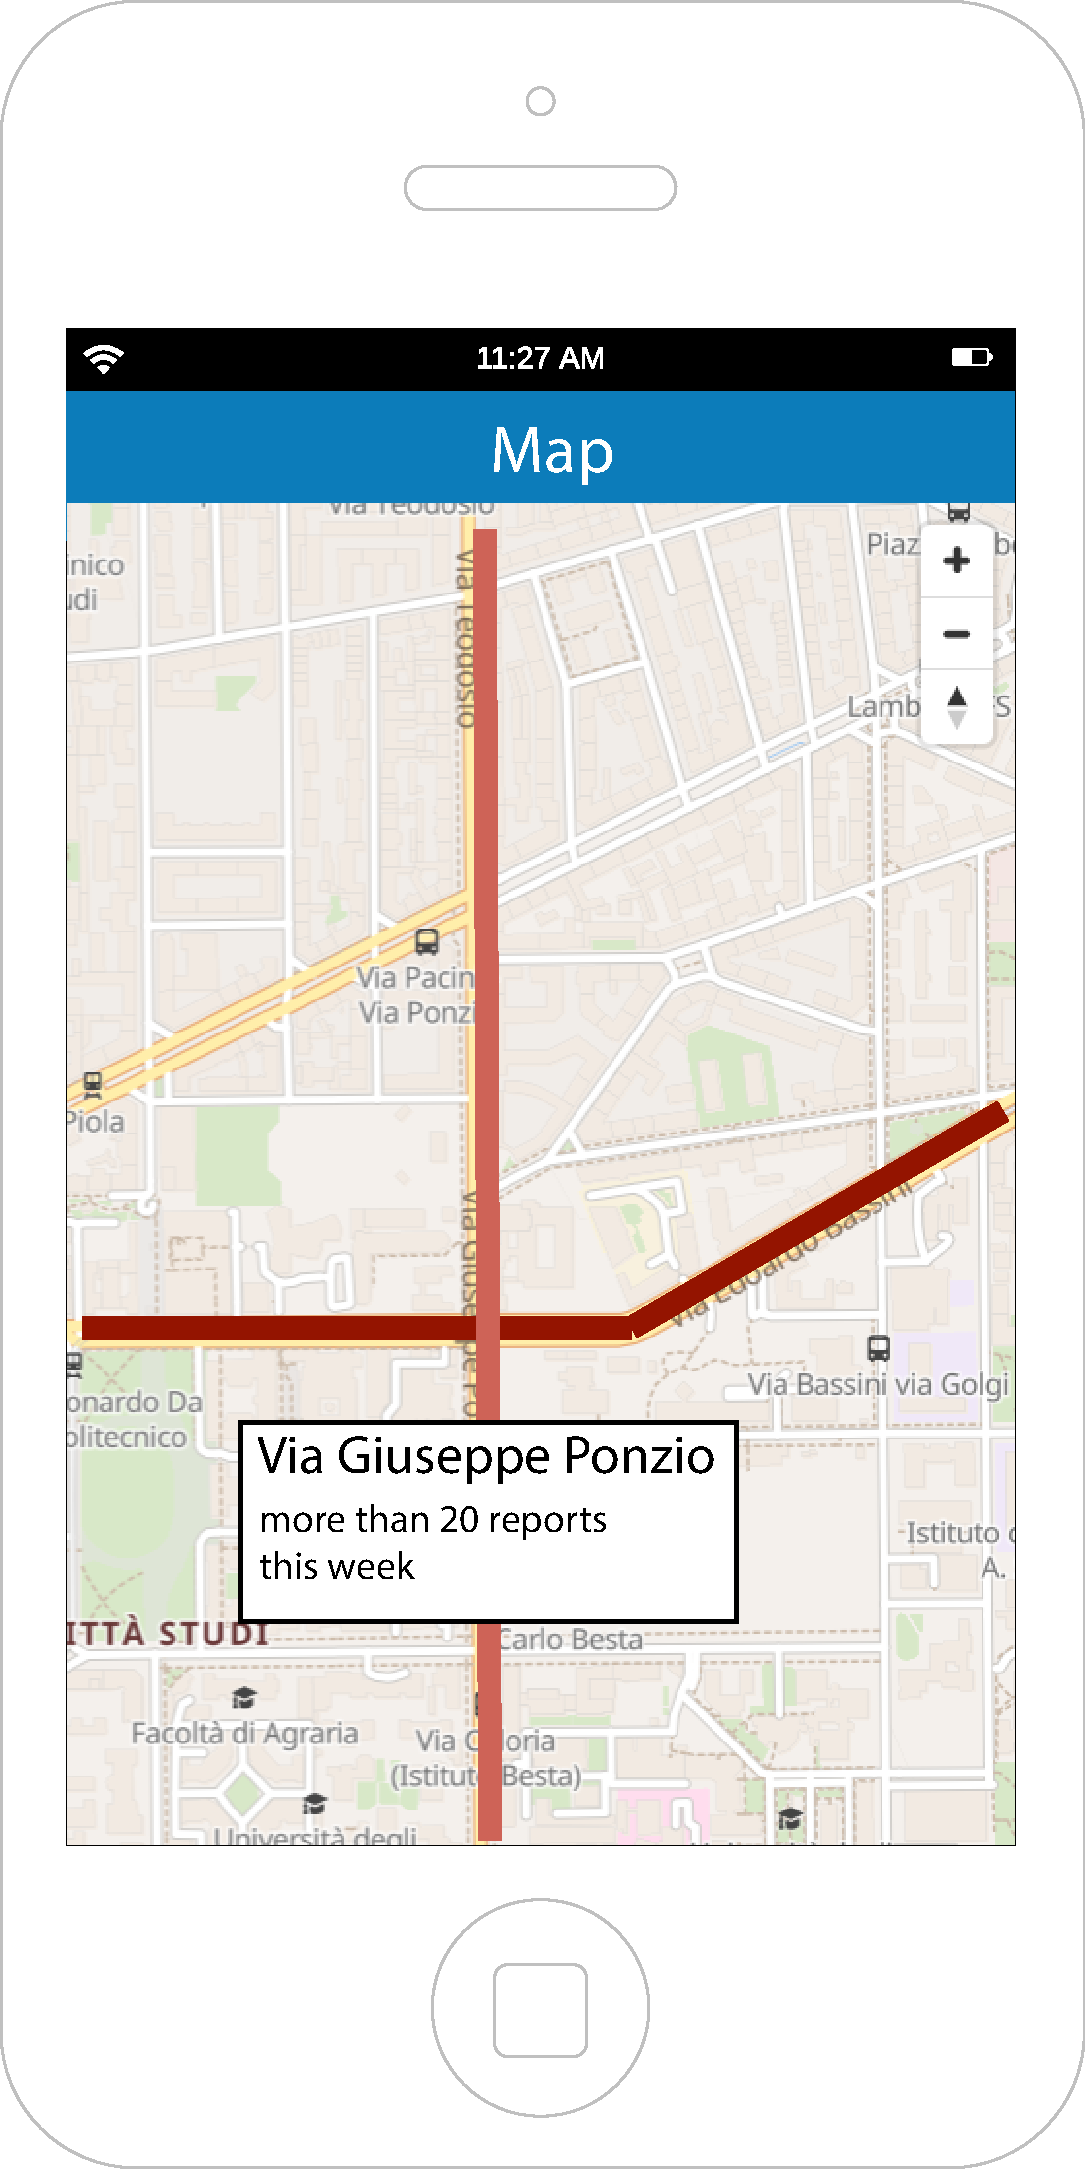
\includegraphics[scale=0.25, center]{Map-detail}
			\caption{User -  map detail}
			\label{fig:subim2}
		\end{subfigure}
		\end{figure}



		\begin{figure}[H]
		\begin{subfigure}{0.5\textwidth}
		\setcounter{subfigure}{6}
			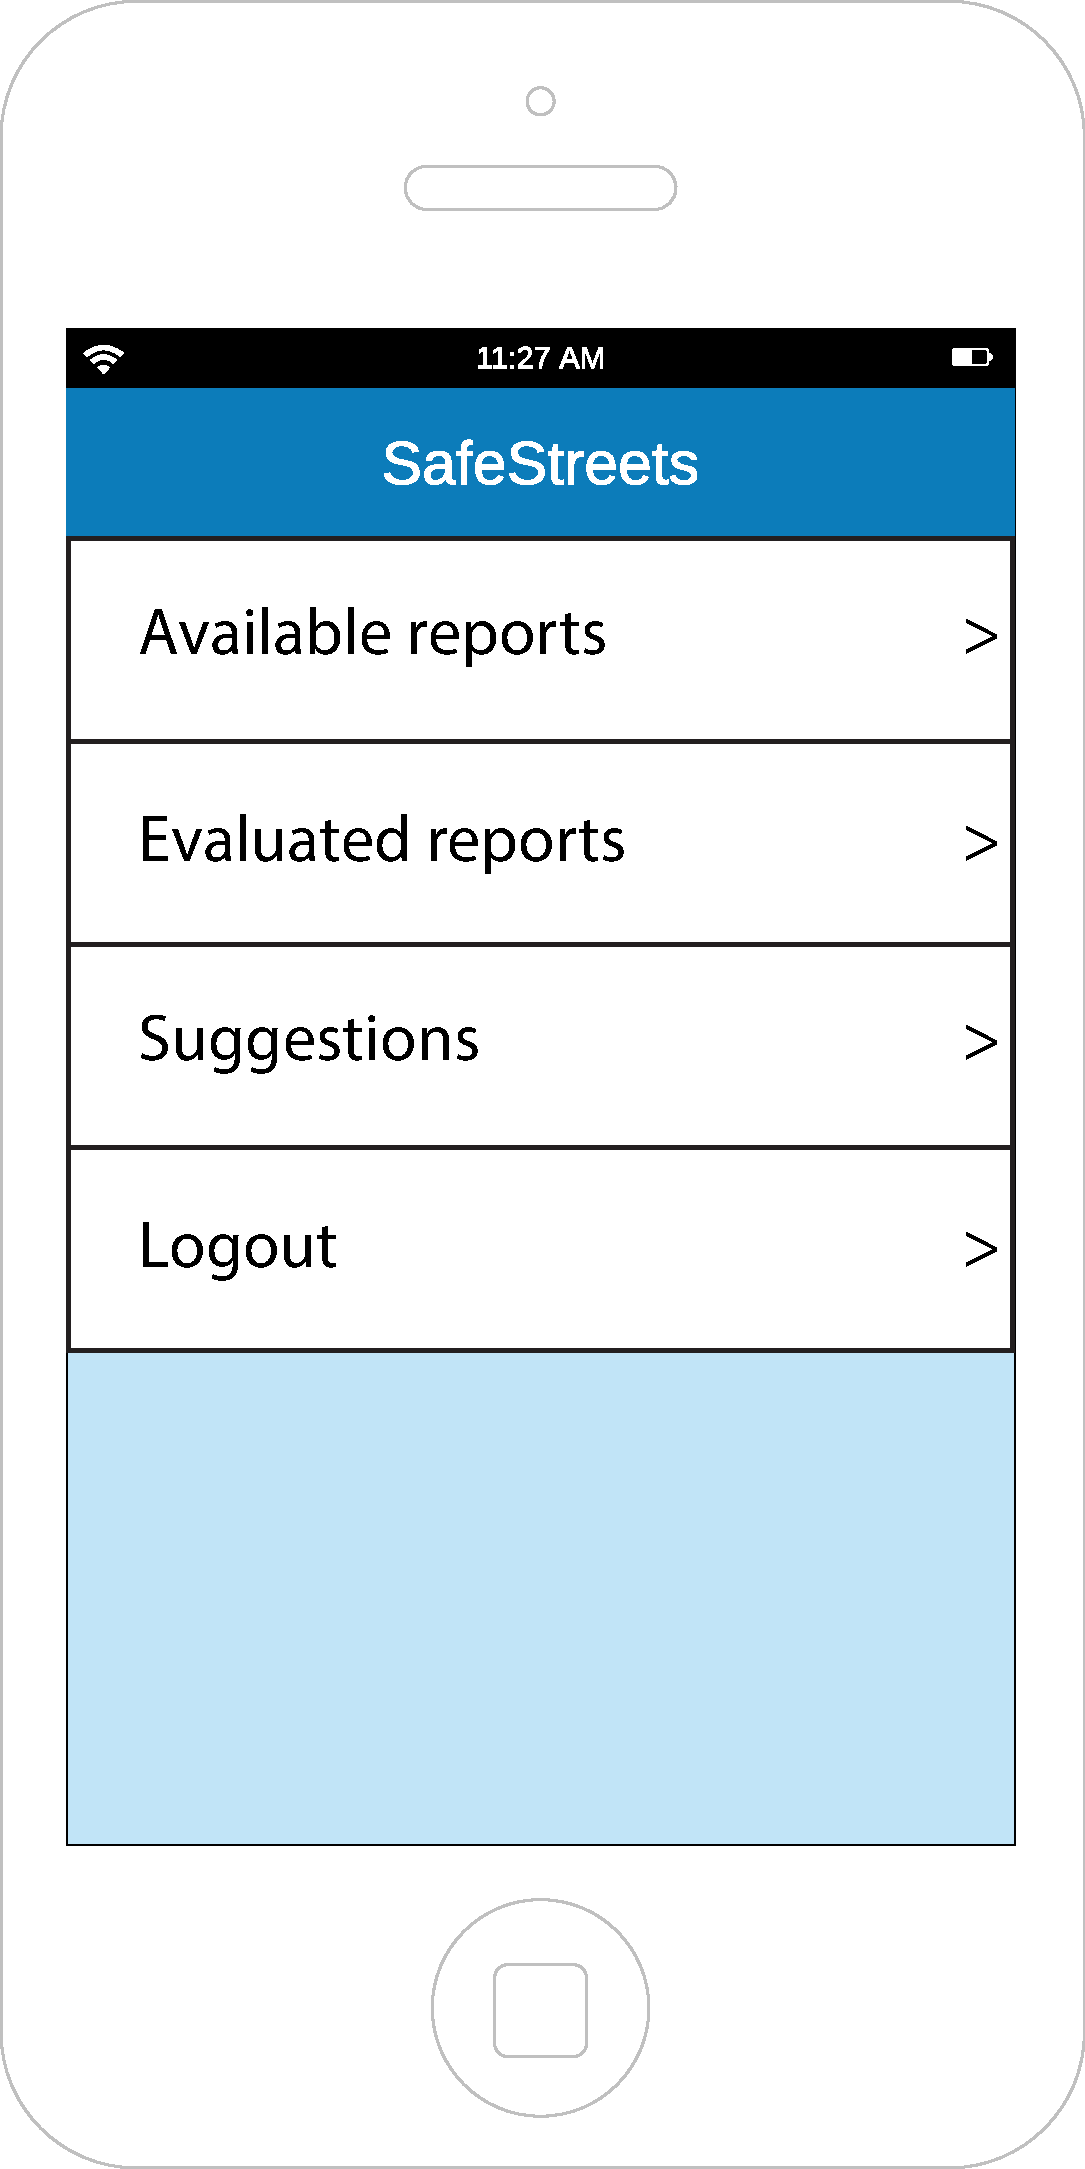
\includegraphics[scale=0.25, center]{HomeAut}
			\caption{Authority - home}
			\label{Authority - home}
		\end{subfigure}
		\begin{subfigure}{0.5\textwidth}
			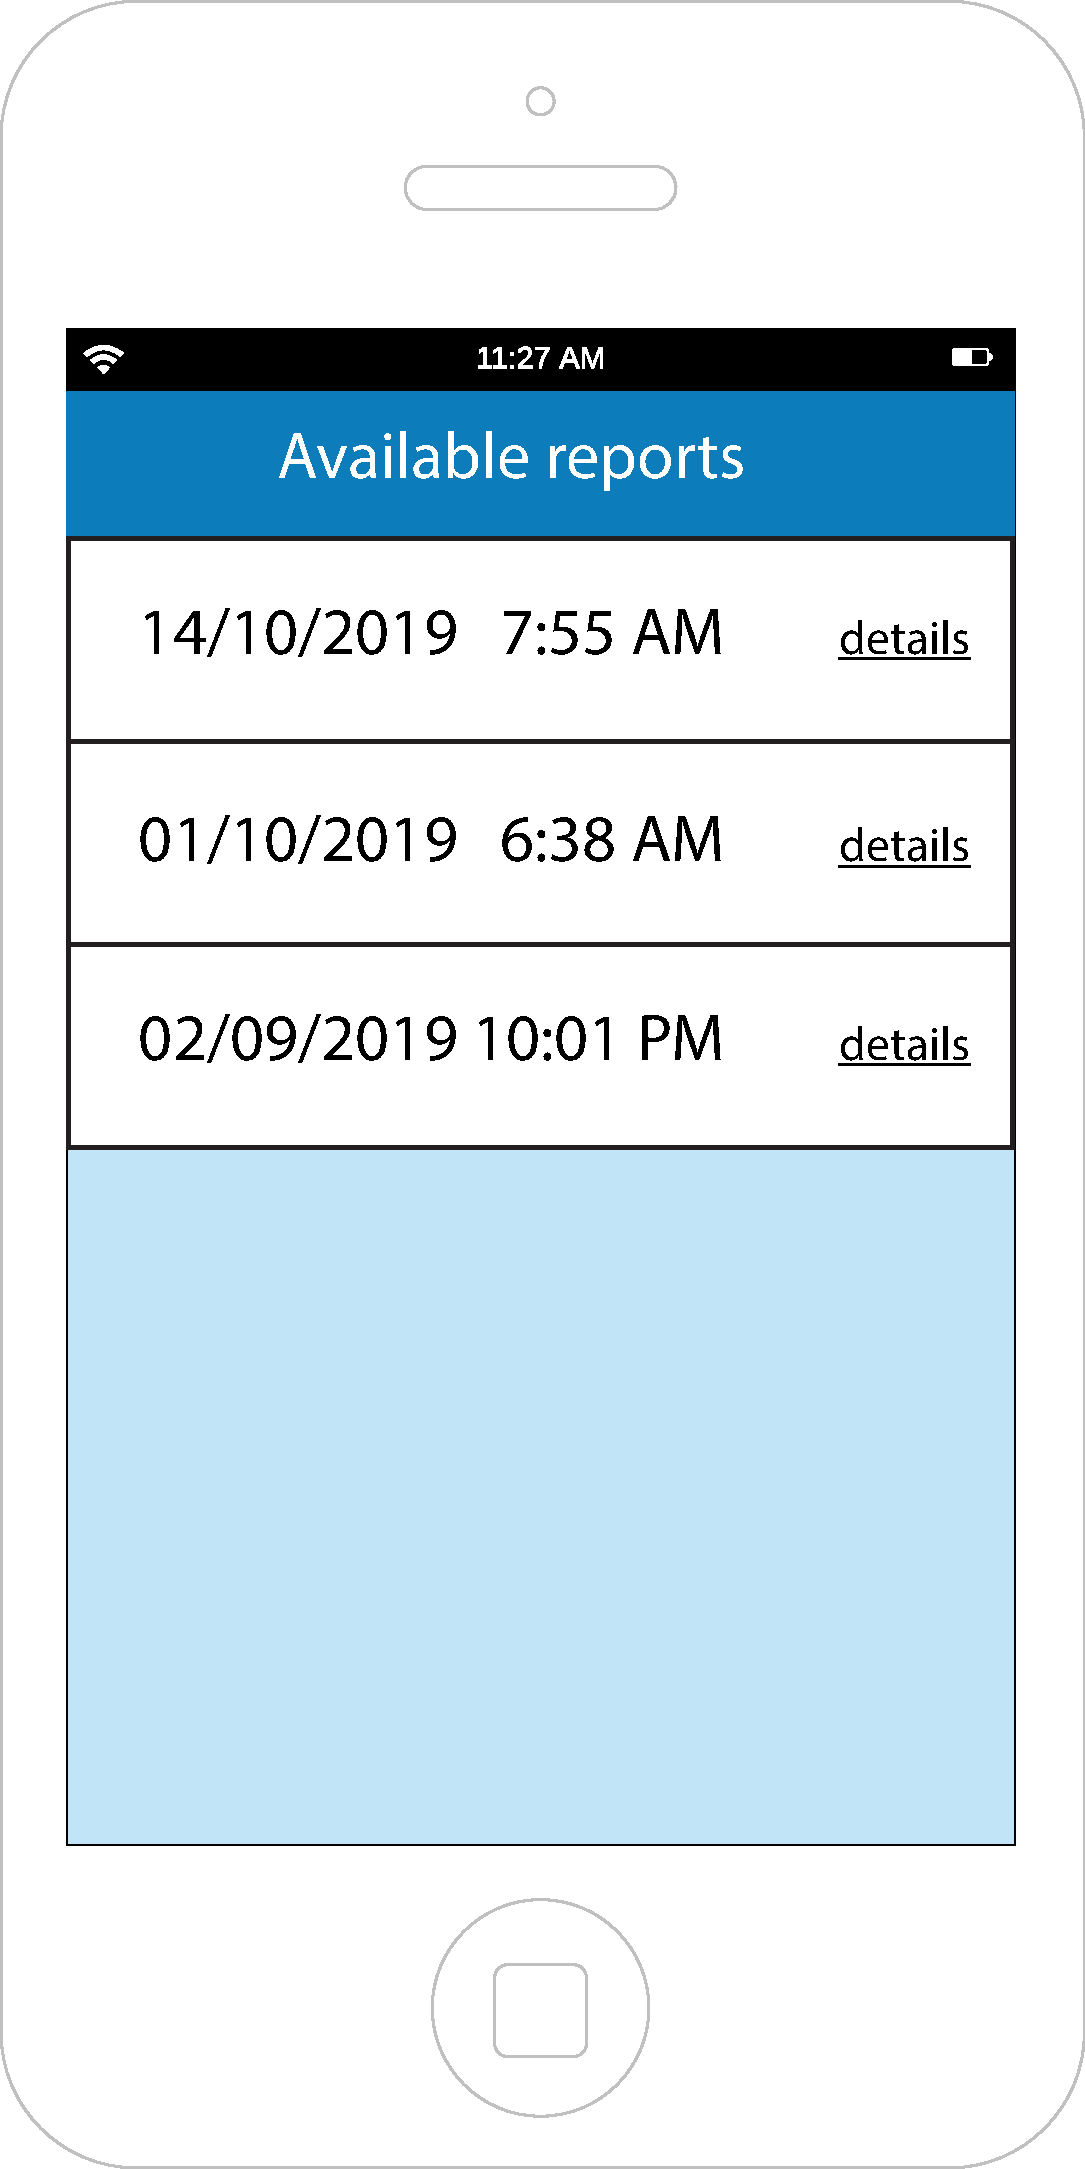
\includegraphics[scale=0.25, center]{Availablereports}
			\caption{Authority - available reports}
			\label{Authority - available reports}
		\end{subfigure}
		\end{figure}
		\begin{figure}[H]
		\begin{subfigure}{0.5\textwidth}
		\setcounter{subfigure}{8}
			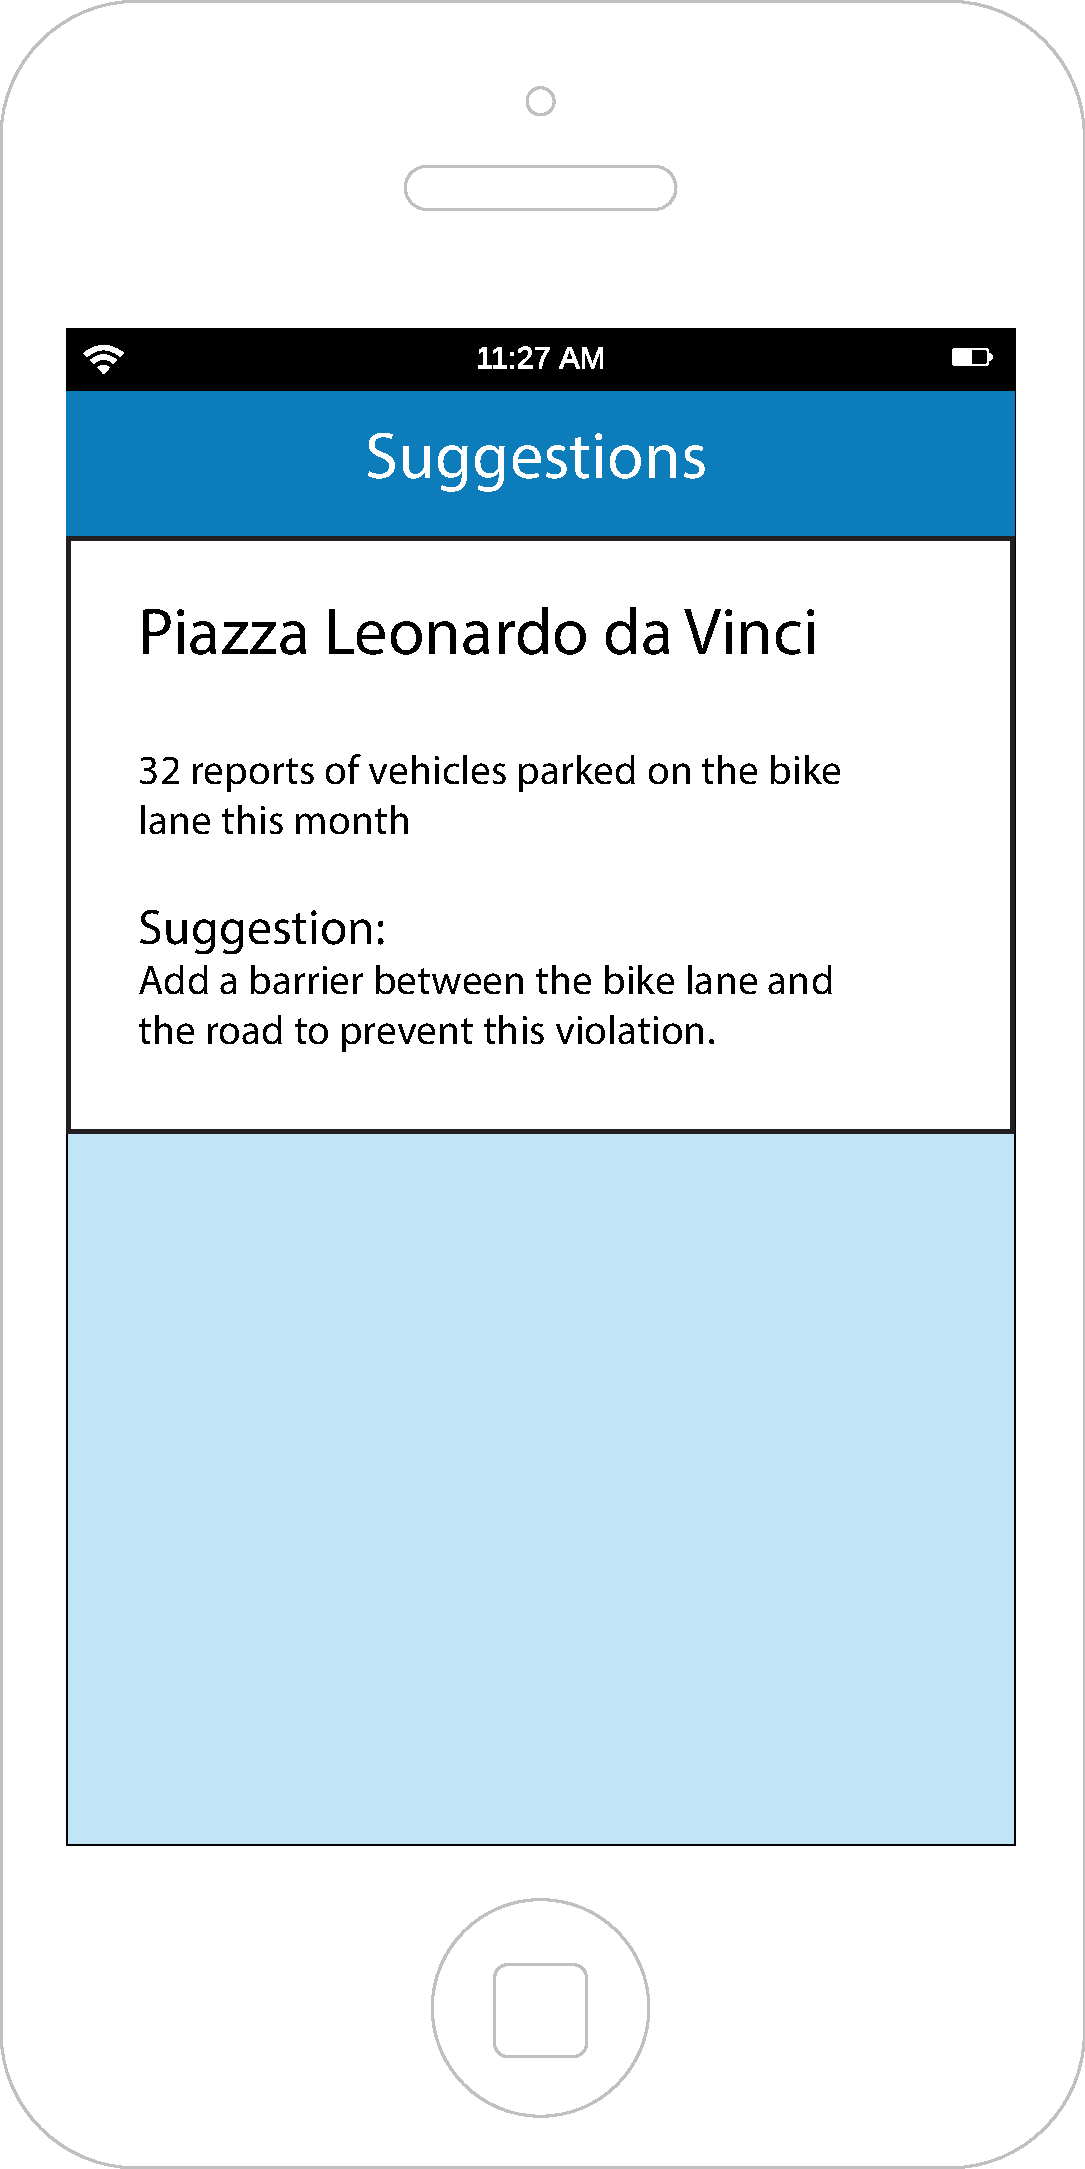
\includegraphics[scale=0.25, center]{Mysuggestions}
			\caption{Authority - suggestion}
			\label{Authority - suggestion}
		\end{subfigure}
		\begin{subfigure}{0.5\textwidth}
			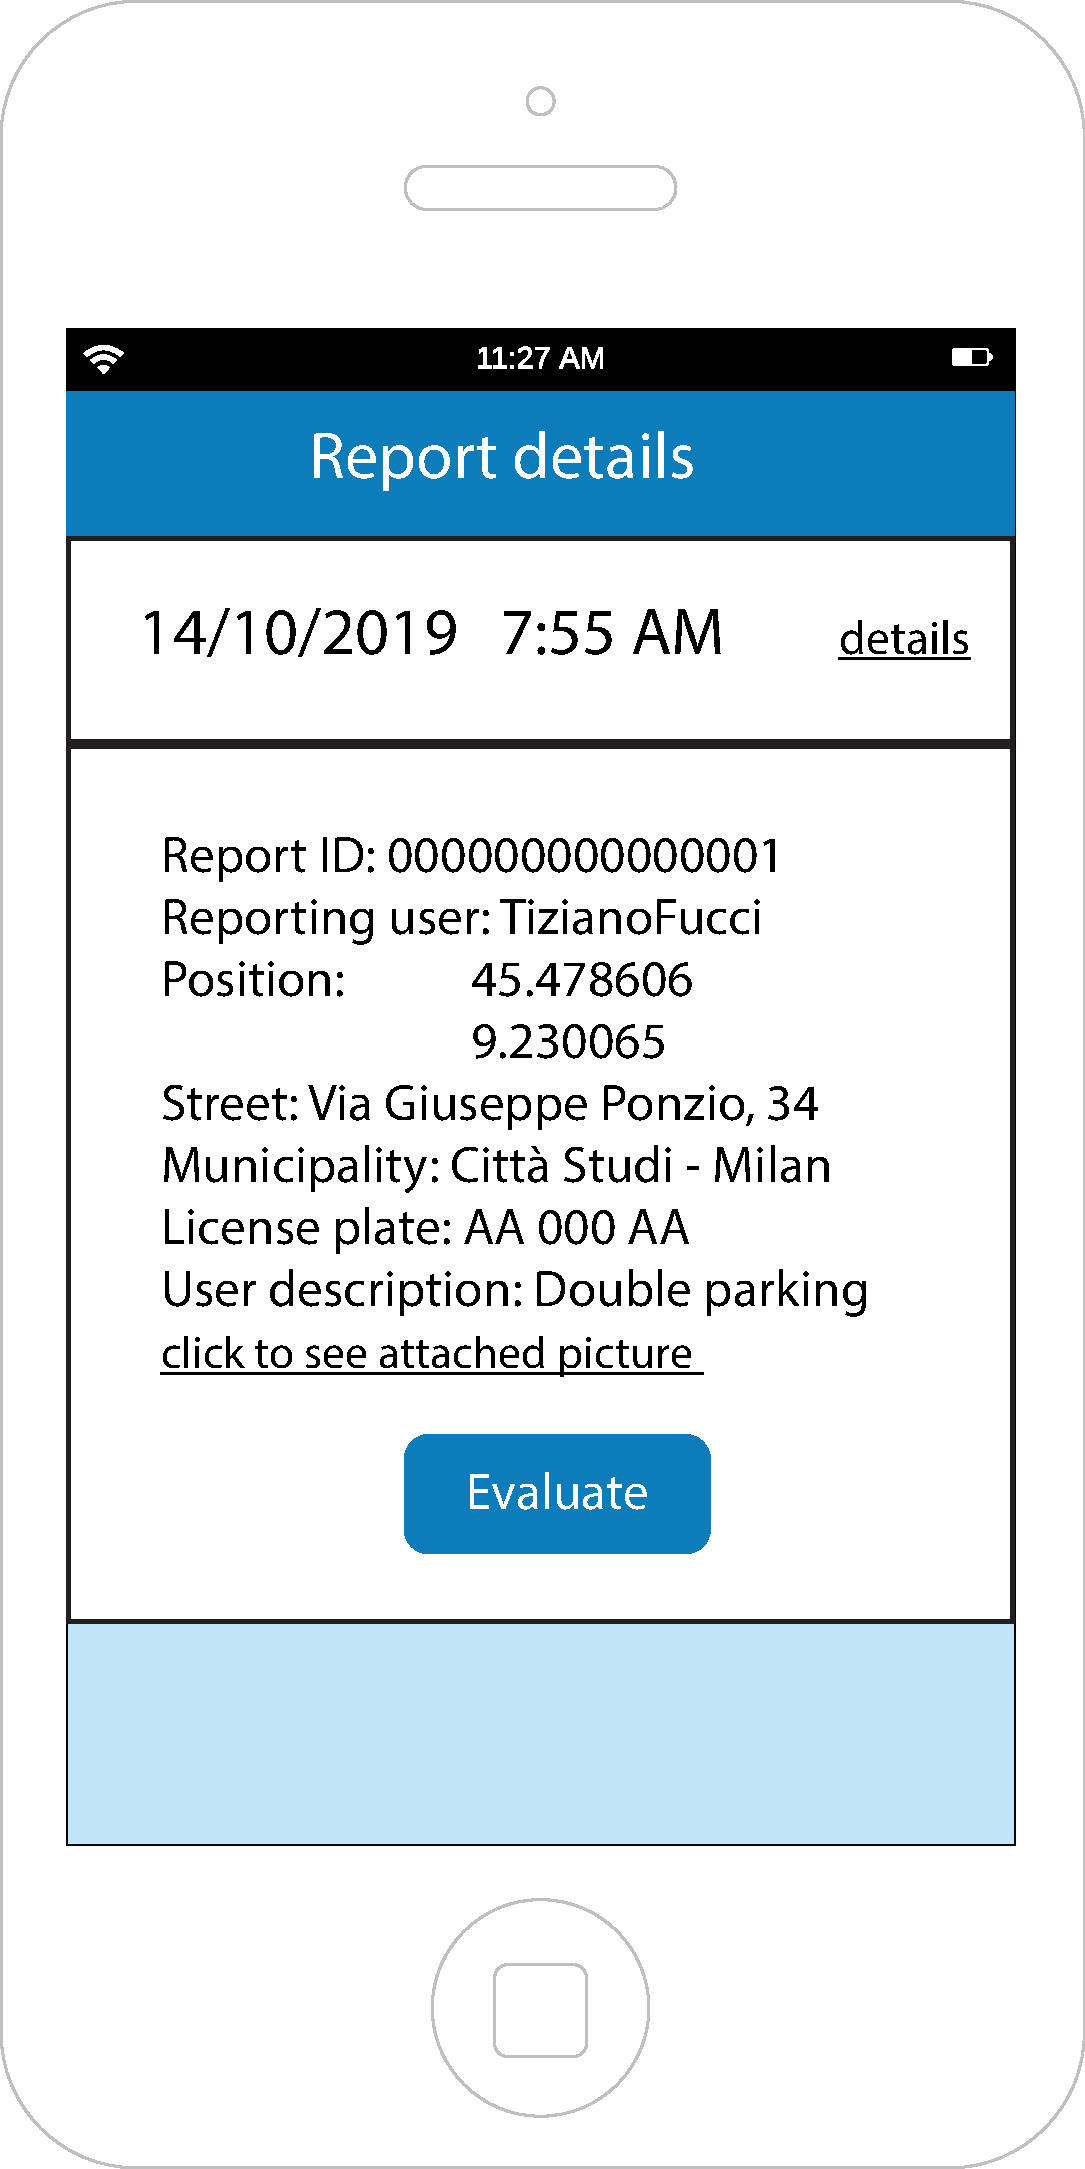
\includegraphics[scale=0.25, center]{Reportdetails}
			\caption{Authority - report details}
			\label{Authority - report details}
		\end{subfigure}
		\end{figure}
		

		\subsection{Hardware interfaces}
			The system has no hardware interfaces.
		\subsection{Software interfaces}
			The system has no software interfaces.
		\subsection{Communication interfaces}
	\section{Functional Requirements}
		This section presents the requirements to be satisfied to reach each goal, in addition to the domain assumptions that must stand.
		\subsection{User} 
			%inizio parte frangi
			\paragraph{Scenarios}
				\subparagraph{Scenario 1}
					Mario, an elderly person who has a reserved parking lot, always has to spend time looking for a free
					car park because someone frequently steals the one reserved to him without being sanctioned by
					authorities. With the help of SafeStreet Mario can report the parking thief to authorities and verify
					that he gets sanctioned.
					
				\subparagraph{Scenario 2}
					Luigi uses very frequently SafeStreet, but he is not sure if what he is doing is considered by authorities,
					thanks to SafeStreets' reports history now he is certain on which reports has been useful and which
					were useless.
					
				\subparagraph{Scenario 3}
					Giuseppe is collecting some data about traffic and traffic violation for an University project, to retrieve more
					information it use the Map offered by SafeStreets to know which zones are more indicated to traffic violations
					
				
				In this paragraph will be illustrated all the use cases diagram, use cases and sequence diagrams.
					
				\begin{figure}[H]
					\begin{subfigure}{\textwidth}
						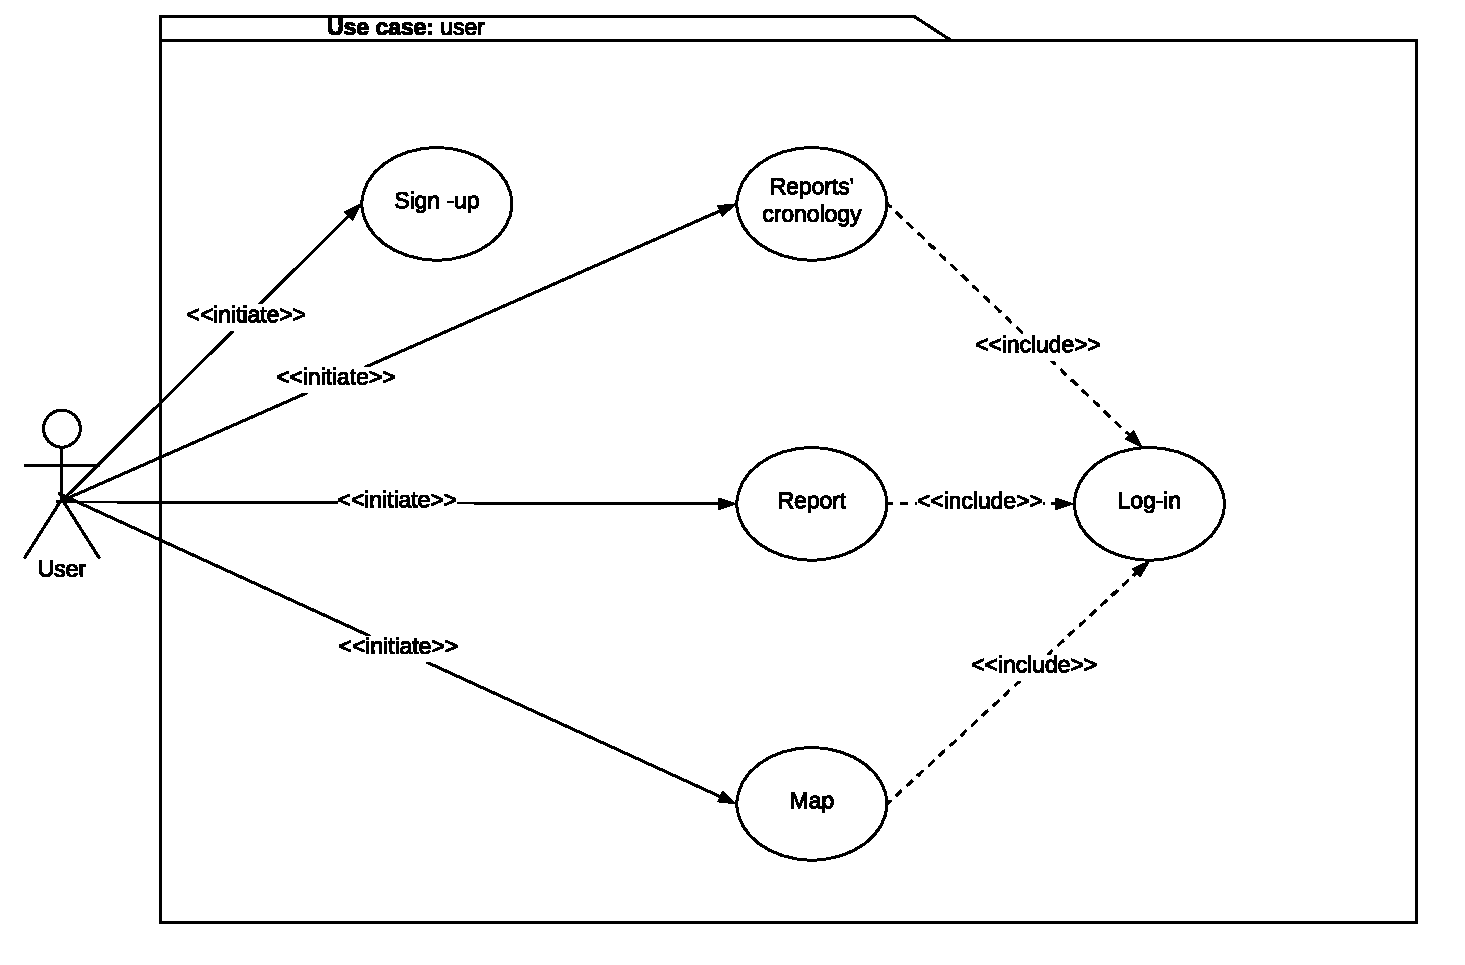
\includegraphics[scale = 0.75, center]{UseCaseC}
						\caption{State diagram on the behavior of reports for citizen}
					\end{subfigure}
				\end{figure}

				\begin{table}[H]
					\centering
					\begin{tabular}{|c|p{0.92\linewidth}|}
						\hline
						Name & {Sign up} \\
						\hline
						Actor & {User, Authorities} \\
						\hline
						Entry condition & {The User want to use for the first time SafeStreet and open the application on
									his device} \\
						\hline
						Events Flows &{ 
								\vskip 4pt
								\begin{enumerate}
									\item The user click on the "Sign up" option
									\item The user fills all the mandatory fields
									\item The user agree with the SafeStreet's privacy policy
									\item The user click the confirmation option
									\item The system proceed to verify user's data and to save them
								\end{enumerate}
								\vskip 4pt}\\
						\hline
						Exit Conditions & {The user is registered and the system has saved his data} \\
						\hline
						Exceptions & {
								\vskip 4pt
								\begin{itemize}
									\item The user has already signed up
									\item Username has been already used. In this case the System notify the user and
										suggests some free Usernames.
									\item The data were not correct. In this case the system ask to the user to check and
										correct eventual mistakes.
									\item Not all the mandatory fields were filled. In this case the system warns the user
										and notify him which fields are empty
								\end{itemize}
								\vskip 4pt
						} \\
						\hline
					\end{tabular}
					\caption{Sing up}
					\label{tab: }
				\end{table}

				\begin{table}[H]
					\centering
					\begin{tabular}{|c|p{0.92\linewidth}|}
						\hline
						Name & {Log in} \\
						\hline
						Actor & {User, Authorities} \\
						\hline
						Entry condition & {The User open the application because he want to access the service he 
									already signed up} \\
						\hline
						Events Flows &{ 
								\vskip 4pt
								\begin{enumerate}
									\item The user click on the "Log in" option
									\item The user fills all the Username and password fields
									\item The user click the confirmation option
									\item The system proceed to verify user's data
									\item The user has free access to the service now
								\end{enumerate}
								\vskip 4pt}\\
						\hline
						Exit Conditions & {The user is logged} \\
						\hline
						Exceptions & {
								\vskip 4pt
								\begin{itemize}
									\item Password wrong
									\item Username wrong, in both case the system will ask to check and correct the 
										log-in information
								\end{itemize}
								\vskip 4pt
						} \\
						\hline
					\end{tabular}
					\caption{Log in}
					\label{tab: }
				\end{table}
				
				\begin{table}[H]
					\centering
					\begin{tabular}{|c|p{0.92\linewidth}|}
						\hline
						Name & {Report} \\
						\hline
						Actor & {User} \\
						\hline
						Entry condition & {The User want to report a traffic violation so open the application and log in,
									then choose the "report" option} \\
						\hline
						Events Flows &{ 
								\vskip 4pt
								\begin{enumerate}
									\item The User clicks on "Report" option
									\item The User take a photo of the violation and the license plate of vehicle
									\item The system tries to understand the plate from the photo
									\item The user check that the system recognized correctly the plate
									\item The user insert the type of violation.
									\item The user clicks on "send report".
									\item The system retrieve device's position and date and time to fill the last fields
										of the report
								\end{enumerate}
								\vskip 4pt}\\
						\hline
						Exit Conditions & {The user reported the violation} \\
						\hline
						Exceptions & {
								\vskip 4pt
								\begin{itemize}
									\item The vehicle has been already reported.
									\item The system cannot obtain the user's position.
									\item Not all the fields has been filled.
									\item There is no internet connection available.
								\end{itemize}
								\vskip 4pt
						} \\
						\hline
					\end{tabular}
					\caption{Report}
					\label{tab: }
				\end{table}

				\begin{table}[H]
					\centering
					\begin{tabular}{|c|p{0.92\linewidth}|}
						\hline
						Name & {Chronology} \\
						\hline
						Actor & {User} \\
						\hline
						Entry condition & {The User open and log in the SafeStreet application} \\
						\hline
						Events Flows &{ 
								\vskip 4pt
								\begin{enumerate}
									\item The user clicks on "History" option
									\item The system searches and sends a recap of all the user's reports
									\item The user can check all his reports
								\end{enumerate}
								\vskip 4pt}\\
						\hline
						Exit Conditions & {The user clicks on "Exit" option} \\
						\hline
						Exceptions & {
								\vskip 4pt
								\begin{itemize}
									\item The user has no reports.
									\item There is no internet connection available.
								\end{itemize}
								\vskip 4pt
						} \\
						\hline
					\end{tabular}
					\caption{Use case Chronology}
					\label{tab: }
				\end{table}
				
				\begin{table}[H]
					\centering
					\begin{tabular}{|c|p{0.92\linewidth}|}
						\hline
						Name & {Visualize Map} \\
						\hline
						Actor & {User} \\
						\hline
						Entry condition & {The User open SafeStreet, log in and choose the "Visualize Map" option} \\
						\hline
						Events Flows &{ 
								\vskip 4pt
								\begin{enumerate}
									\item The user click on "Visualize Map"
									\item The system retrieve the device's position and obtain information about
										the near streets' reports number to calculate their "level" and display
										it correctly
									\item The user can navigate in the map seeing each street and their level
								\end{enumerate}
								\vskip 4pt}\\
						\hline
						Exit Conditions & {The user clicks on exit button} \\
						\hline
						Exceptions & {
								\vskip 4pt
								\begin{itemize}
									\item There is no internet connection
									\item The GPS system is not functioning
									\item The app doesn't have permits to access to device's position
								\end{itemize}
								\vskip 4pt
						} \\
						\hline
					\end{tabular}
					\caption{Use case on Visualize Map}
					\label{tab: }
				\end{table}
				
				\begin{figure}[H]
					\begin{subfigure}{\textwidth}
						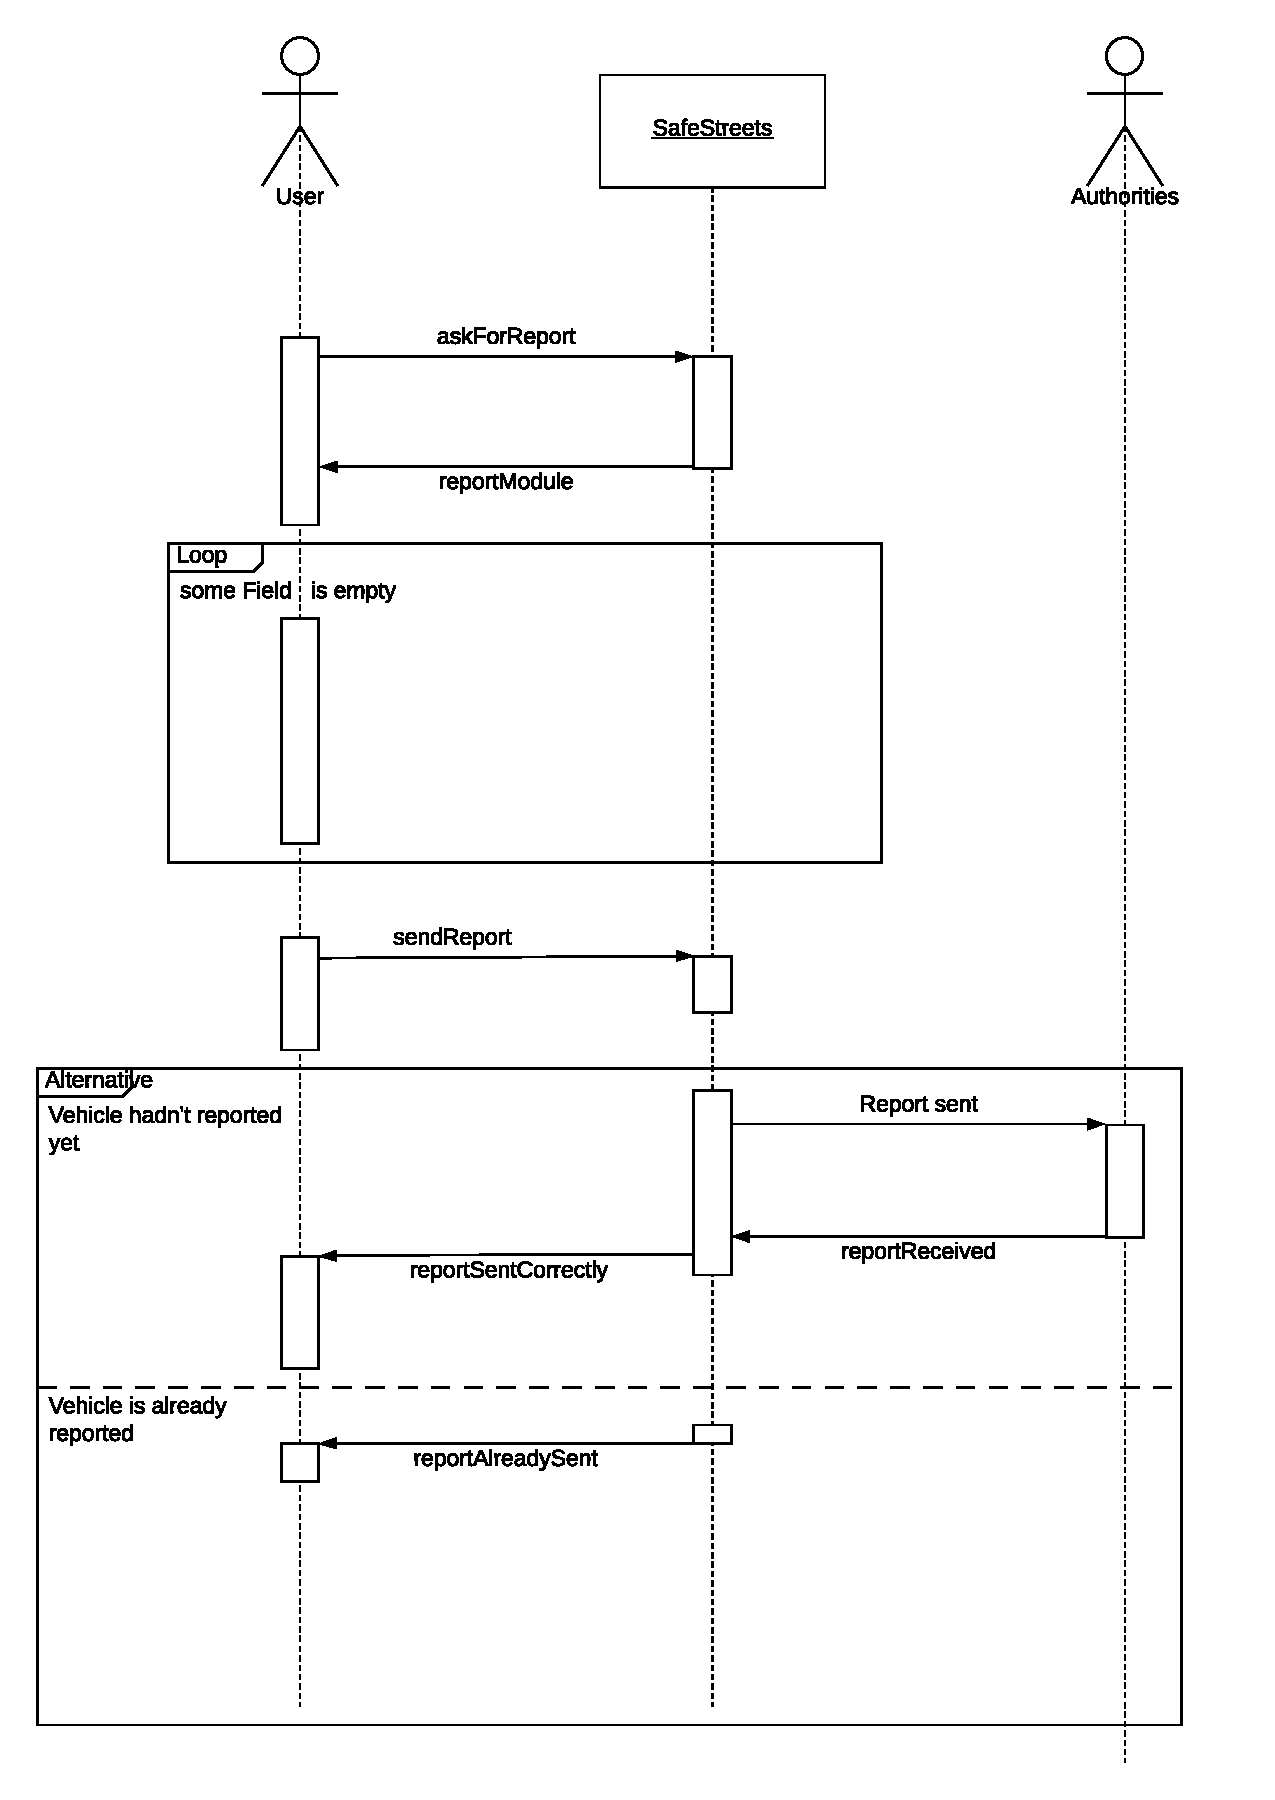
\includegraphics[scale = 0.75, center]{ReportSequenceDiagram}
						\caption{Sequence diagram on the behavior of reports for citizen}
					\end{subfigure}
				\end{figure}
				\begin{figure}[H]
					\begin{subfigure}{\textwidth}
						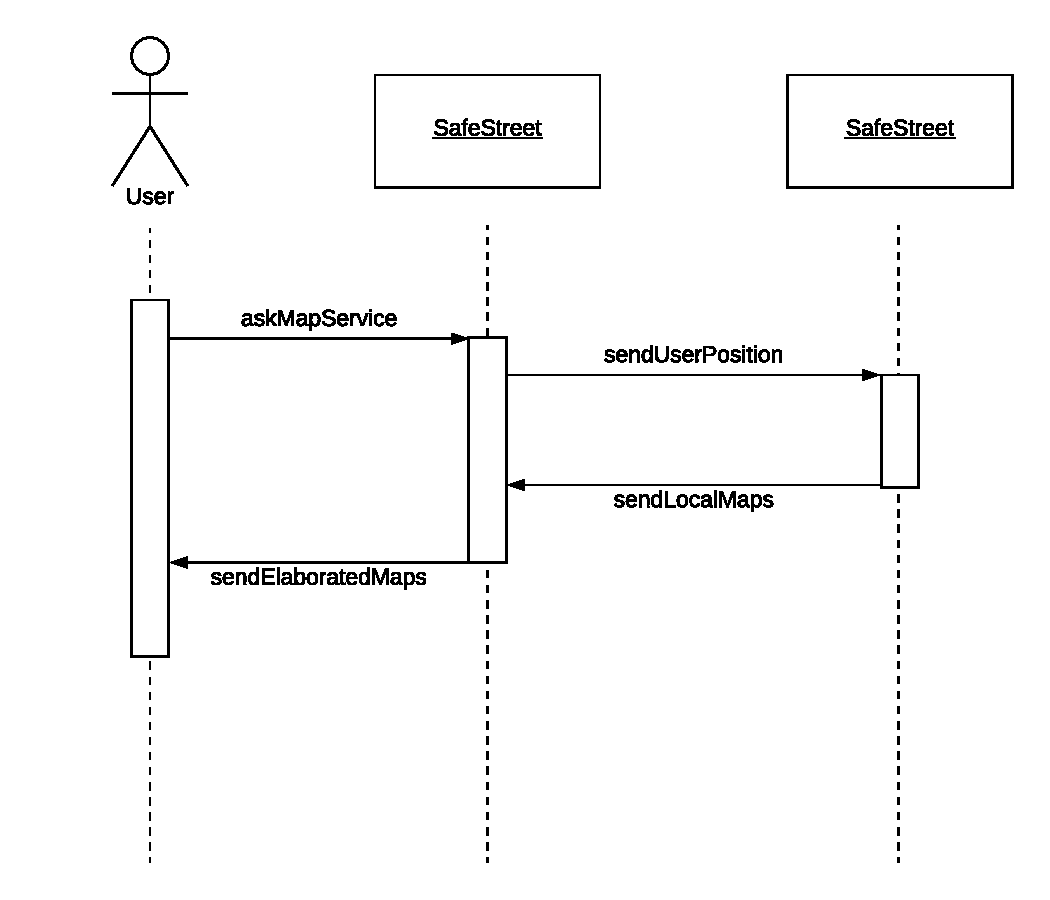
\includegraphics[scale = 0.70, center]{MapSequenceDiagram}
						\caption{Sequence diagram about Map option}
					\end{subfigure}
				\end{figure}
				\begin{figure}[H]
					\begin{subfigure}{\textwidth}
						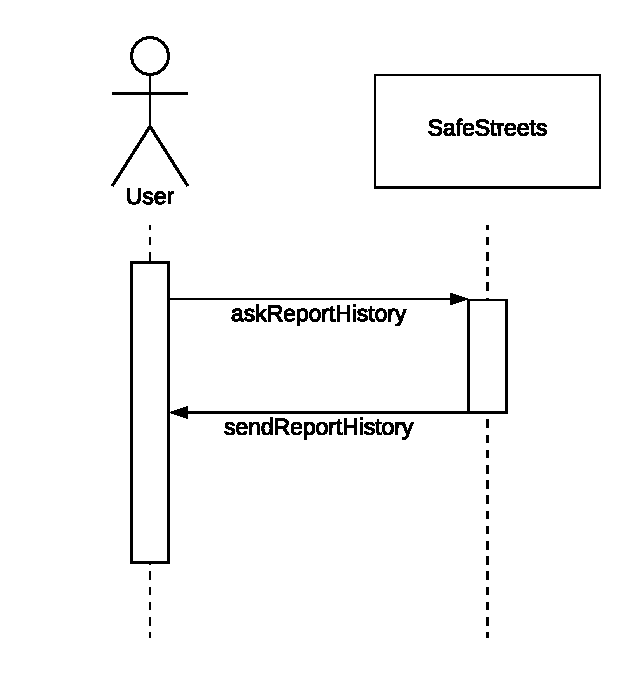
\includegraphics[scale = 0.70, center]{HhistorySequenceDiagram}
						\caption{Reports History}
					\end{subfigure}
				\end{figure}
			%fine
			
			
			
			\paragraph {G1:} The application must allow the users to register entering an e-mail address and a password.
			\begin{itemize}
				\item{[R1]:} Registration must be allowed only entering an e-mail address that is not already associated to an existing SafeStreets account.
				\item{[R2]:} Registration must be allowed only entering a password that satisfies the safety conditions.
				\item{[R8]:} The system must store the hash of every password, using a safe cryptographic hash function.
			\end{itemize}

			\paragraph {G2:} The application must allow the users to notify traffic violations, providing the type of violation and a picture of the vehicle.
			\begin{itemize}
				\item{[D1]:} The users always provide a picture that allows both the algorithm to read the license plate and the authority to identify the violation.
				\item{[D2]:} Every user is provided with a device capable to share the exact GPS position at any moment.
				\item{[D3]:} Every user is provided with a device capable to share the exact GPS position at any moment.
				\item{[D5]:} Date, time and street of the violation are automatically inferred by the application.
				\item{[D6]:} The user sends the report staying in the same place of the violation attached to the report.
		 		\item{[D7]:} : The picture of the license plate is taken at the moment and shows the right car.
			\end{itemize}
			\begin{itemize}
				\item{[R1]:} The system must check if the location of the report belongs to some municipality exploiting SafeStreets.
				\item{[R2]:} The system must add the right date, time and street of the violation to the data provided by the user.
				\item{[R3]:} The system must correctly read the license plate given a picture attached to a report.
			\end{itemize}

			\paragraph {G3:} The application must be able to show to the users the streets and the vehicles with the highest frequency of violations.
			\begin{itemize}
				\item{[D3]:} The name of the street where a violation occured is retrieved from the GPS position.
				\item{[D4]:} Authorities never make mistakes in evaluating a report.
				\item{[D5]:} Reports are evaluated only one time.
			\end{itemize}
			\begin{itemize}
				\item{[R2]:} The system must add the right date, time and street of the violation to the data provided by the user.
				\item{[R4]:} The system must exploit Google Maps APIs to show to the user the map of the violations.
				\item{[R5]:} The system must show the right colors on the map, given the number of approved reports for each street.
				\item{[R6]:} When a license plate is recognized, the system must show the number of approved reports for that car.
				\item{[R9]:} If the same violation is reported twice, it counts only one time on the map.
			\end{itemize}
				\paragraph {G4:}  The application must allow the user to see all of his reports and their status.
			\begin{itemize}
				\item{[R2]:} The system must add the right date, time and street of the violation to the data provided by the user.
				\item{[R7]:} The system must assign to each report a unique identification number.
			\end{itemize}
			\paragraph {G5:} The system must notify the user when one of his reports is evaluated.
			\begin{itemize}
				\item{[D3]:} The name of the street where a violation occured is retrieved from the GPS position.
				\item{[D4]:} Authorities never make mistakes in evaluating a report.
				\item{[D5]:} Reports are evaluated only one time.
			\end{itemize}
			\begin{itemize}
				\item{[R2]:} The system must add the right date, time and street of the violation to the data provided by the user.
				\item{[R4]:} The system must exploit Google Maps APIs to show to the user the map of the violations.
				\item{[R5]:} The system must show the right colors on the map, given the number of approved reports for each street.
				\item{[R6]:} When a license plate is recognized, the system must show the number of approved reports for that car.
				\item{[R9]:} If the same violation is reported twice, it counts only one time on the map.
			\end{itemize}
			
		\subsection{Authority}
			
			\paragraph {G6:} The application must allow the authorities to register providing a valid identification number and a valid password.
				\begin{itemize}
					\item{[R1]:} Registration must be allowed only entering an e-mail address that is not already associated to an existing SafeStreets account.
					\item{[R2]:} Registration must be allowed only entering a password that satisfies the safety conditions.
					\item{[R8]:} The system must store the hash of every password, using a safe cryptographic hash function.
				\end{itemize}

			\paragraph {G7:} The application must allow authorities to retrieve and evaluate the available reports.
				\begin{itemize}
					\item{[D3]:} The name of the street where a violation occured is retrieved from the GPS position.
					\item{[D5]:} Reports are evaluated only one time.
				\end{itemize}
				\begin{itemize}
					\item{[R1]:} The system must check if the location of the report belongs to some municipality exploiting SafeStreets.
					\item{[R2]:} The system must add the right date, time and street of the violation to the data provided by the user.
					\item{[R7]:} The system must assign to each report a unique identification number.
					\item{[R10:]} The system must guarantee that each municipality is covered by at least one authority.
					\item{[R12]:} The system must notify the authorities when a new report is available.
				\end{itemize}
			\paragraph {G8:} The application must be able to identify potentially unsafe areas and suggest possible interventions.
				\begin{itemize}
					\item{[D3]:} Every user is provided with a device capable to share the exact GPS position at any moment.
			 		\item{[D4]:} Authorities never make mistakes in evaluating a report.
					\item{[D5]:} Date, time and street of the violation are automatically inferred by the application.
			 		\item{[D6]:} The user sends the report staying in the same place of the violation.
				\end{itemize}
				\begin{itemize}
					\item{[R9]:} If the same violation is reported twice, it counts only one time on the map.
					\item{[R10:]} The system must guarantee that each municipality is covered by at least one authority.
					\item{[R11]:} The system must include a simple recommender system that, according on the number of each type of violation, suggests a possible intervention to the authorities of a municipality.
				\end{itemize}
\paragraph{Scenarios}
				\subparagraph{Scenario 1}
					Eddie Edison, an officer had noticed a vertiginous increment of traffic violations, so to increase the control
					on the streets decide to join SafeStreets
					
				\subparagraph{Scenario 2}
					Major Clancy Winchester had noticed that even with various tentative to reduce the car accidents he didn't
					succeed, so he decide to try to subscribe to and advanced option offered by SafeStreets trying to receive
					new suggestion to improve the security
					
				In this paragraph will be illustrated all the use cases diagram, use cases and sequence diagrams, the "sing up" and "log in"
				are not reported because are the same as above.
			
			\begin{figure}[H]
				\begin{subfigure}{\textwidth}
					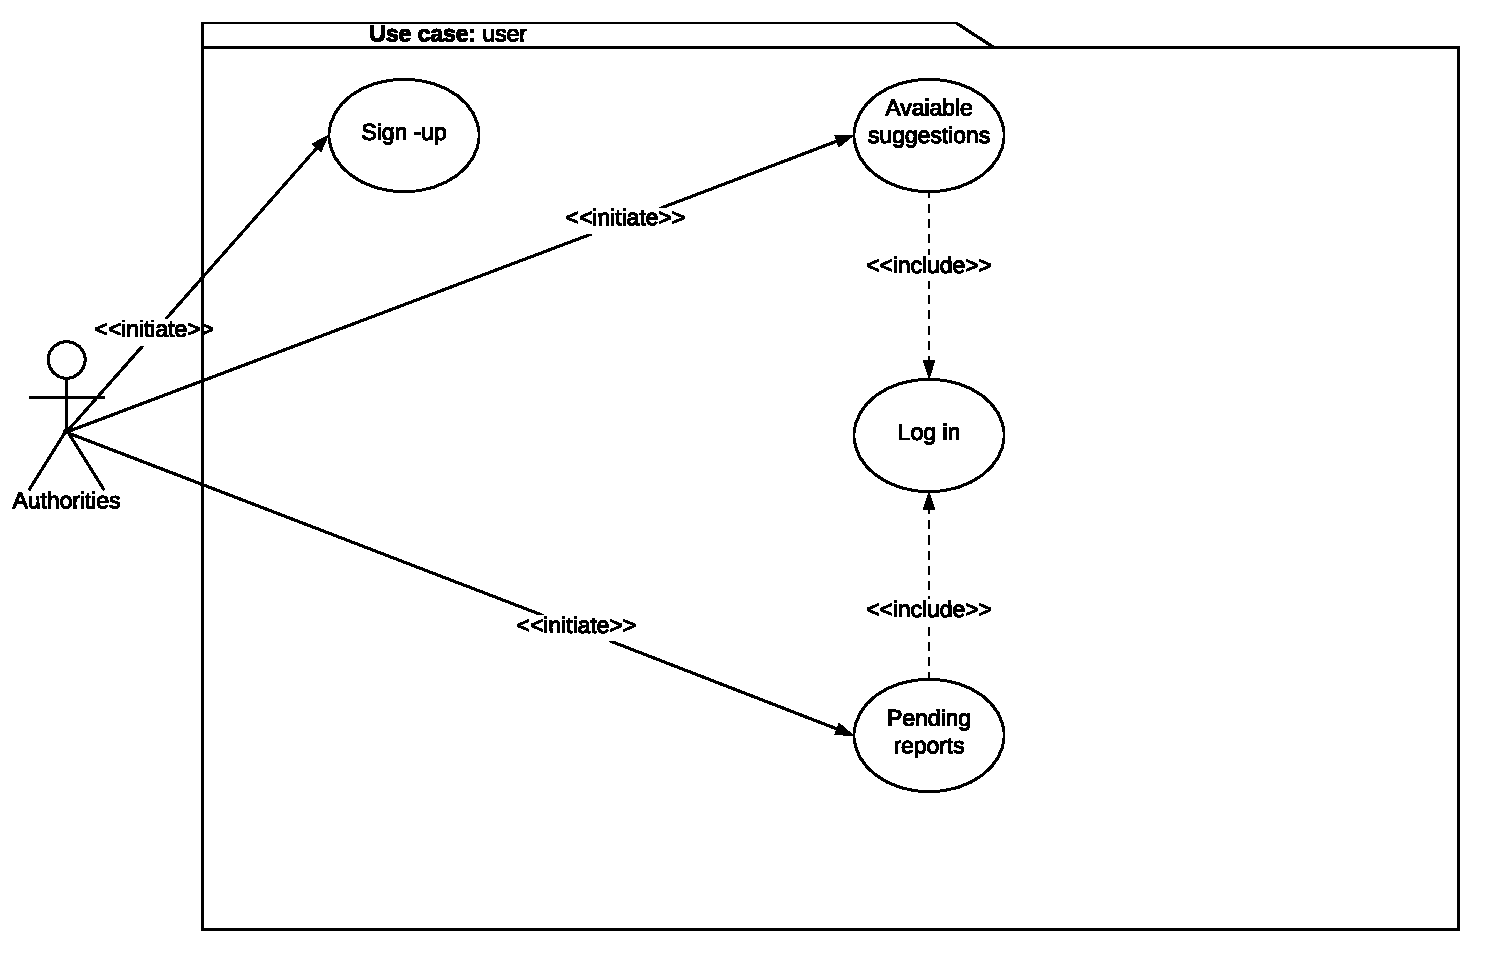
\includegraphics[scale = 0.75, center]{UseCaseA}
					\caption{Sequence diagram on the behavior of reports for citizen}
				\end{subfigure}
			\end{figure}
			

			\begin{table}[H]
				\centering
				\begin{tabular}{|c|p{0.92\linewidth}|}
					\hline
					Name & {Evaluate report} \\
					\hline
					Actor & {Authorities} \\
					\hline
					Entry condition & {The authorities is logged in} \\
					\hline
					Events Flows &{ 
							\vskip 4pt
							\begin{enumerate}
								\item The authority click on the "Evaluate reports" options
								\item The system retrieve all the pending reports
								\item The authority choose if accept or reject each single report based on the information
									contained in the report
							\end{enumerate}
							\vskip 4pt}\\
					\hline
					Exit Conditions & {The user clicks on exit button} \\
					\hline
					Exceptions & {/} \\
					\hline
				\end{tabular}
				\caption{Evaluate report}
				\label{tab: }
			\end{table}
			
			\begin{table}[H]
				\centering
				\begin{tabular}{|c|p{0.92\linewidth}|}
					\hline
					Name & {Suggestion} \\
					\hline
					Actor & {Authorities} \\
					\hline
					Entry condition & {The authorities is logged in} \\
					\hline
					Events Flows &{ 
							\vskip 4pt
							\begin{enumerate}
								\item The authority click on the "Suggestion" options
								\item He choose one Street under his control
								\item The system based on the street and the accidents give a recommendation
							\end{enumerate}
							\vskip 4pt}\\
					\hline
					Exit Conditions & {The user clicks on exit button} \\
					\hline
					Exceptions & {The authorities hasn't activated this optional functionality} \\
					\hline
				\end{tabular}
				\caption{Evaluate report}
				\label{tab: }
			\end{table}
			
			\begin{figure}[H]
				\begin{subfigure}{\textwidth}
					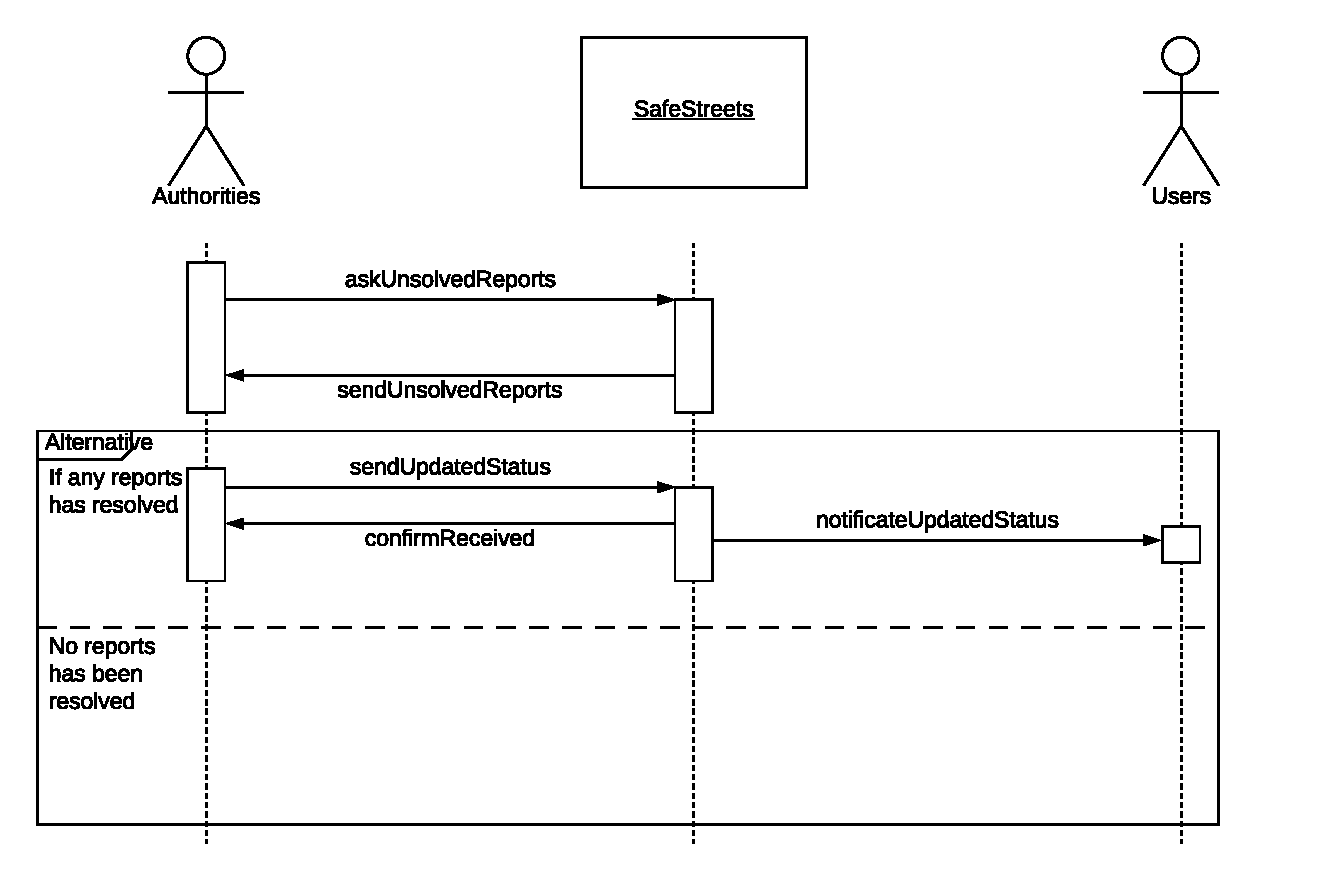
\includegraphics[scale = 0.75, center]{EvaluateSequenceDiagram}
					\caption{Sequence diagram on the behavior of reports for citizen}
				\end{subfigure}
			\end{figure}

			\begin{figure}[H]
				\begin{subfigure}{\textwidth}
					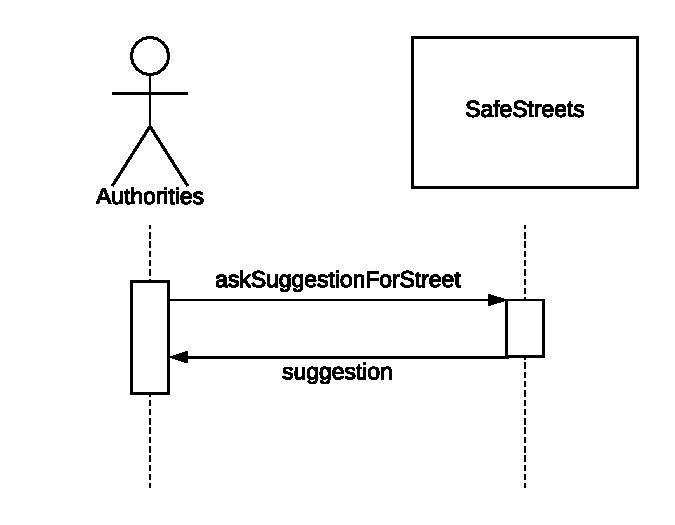
\includegraphics[scale = 0.75, center]{SuggestionSequenceDiagram}
					\caption{Sequence diagram on the behavior of reports for citizen}
				\end{subfigure}
			\end{figure}



	
	\section{Performance Requirments}
	\section{Design constraints}
		\subsection{Standards compliance}
		\subsection{Hardware limitations}
		\subsection{Any other costraint}
	\section{Software System Attributes}
		\subsection{Reliability}
		\subsection{Availability}
		\subsection{Security}
		\subsection{Maintainability}
		\subsection{Portablity}
% End of third chapter

\chapter{Formal Analysis}
	\section{Purpose}
This chapter shows the analysis of the Alloy model of the proposed system. Obviously, here the focus is only on some critical aspects of the application that require a special attention. In particular, the purpose of this model is to guarantee that:
\begin{itemize}
	\item The provided e-mail address is different for each user or authority;
	\item Every report has a unique identification number;
	\item Every municipality has at least one authority assigned;
	\item The authorities correctly receive notifications when a report is available;
	\item The users correctly receive notifications when one of their report is evaluated.
\end{itemize}
	\section{Model}

	\lstinputlisting[language=alloy]{Model.als}

	\section{Results}
	The following is the result of the Alloy Analizer with the input shown in the previous section. The \emph{world1} predicate is used to generate a world suitable to be read, which will be shown in the next section.
		\begin{figure}[H]
				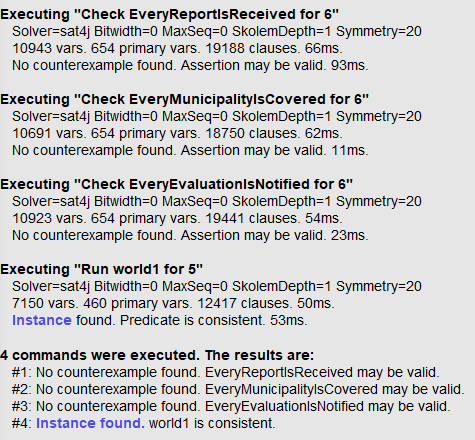
\includegraphics[scale = 0.9, center]{Consistency}
				\caption{Results}
		\end{figure}

	\section{Generated world}
		\begin{figure}[H]
				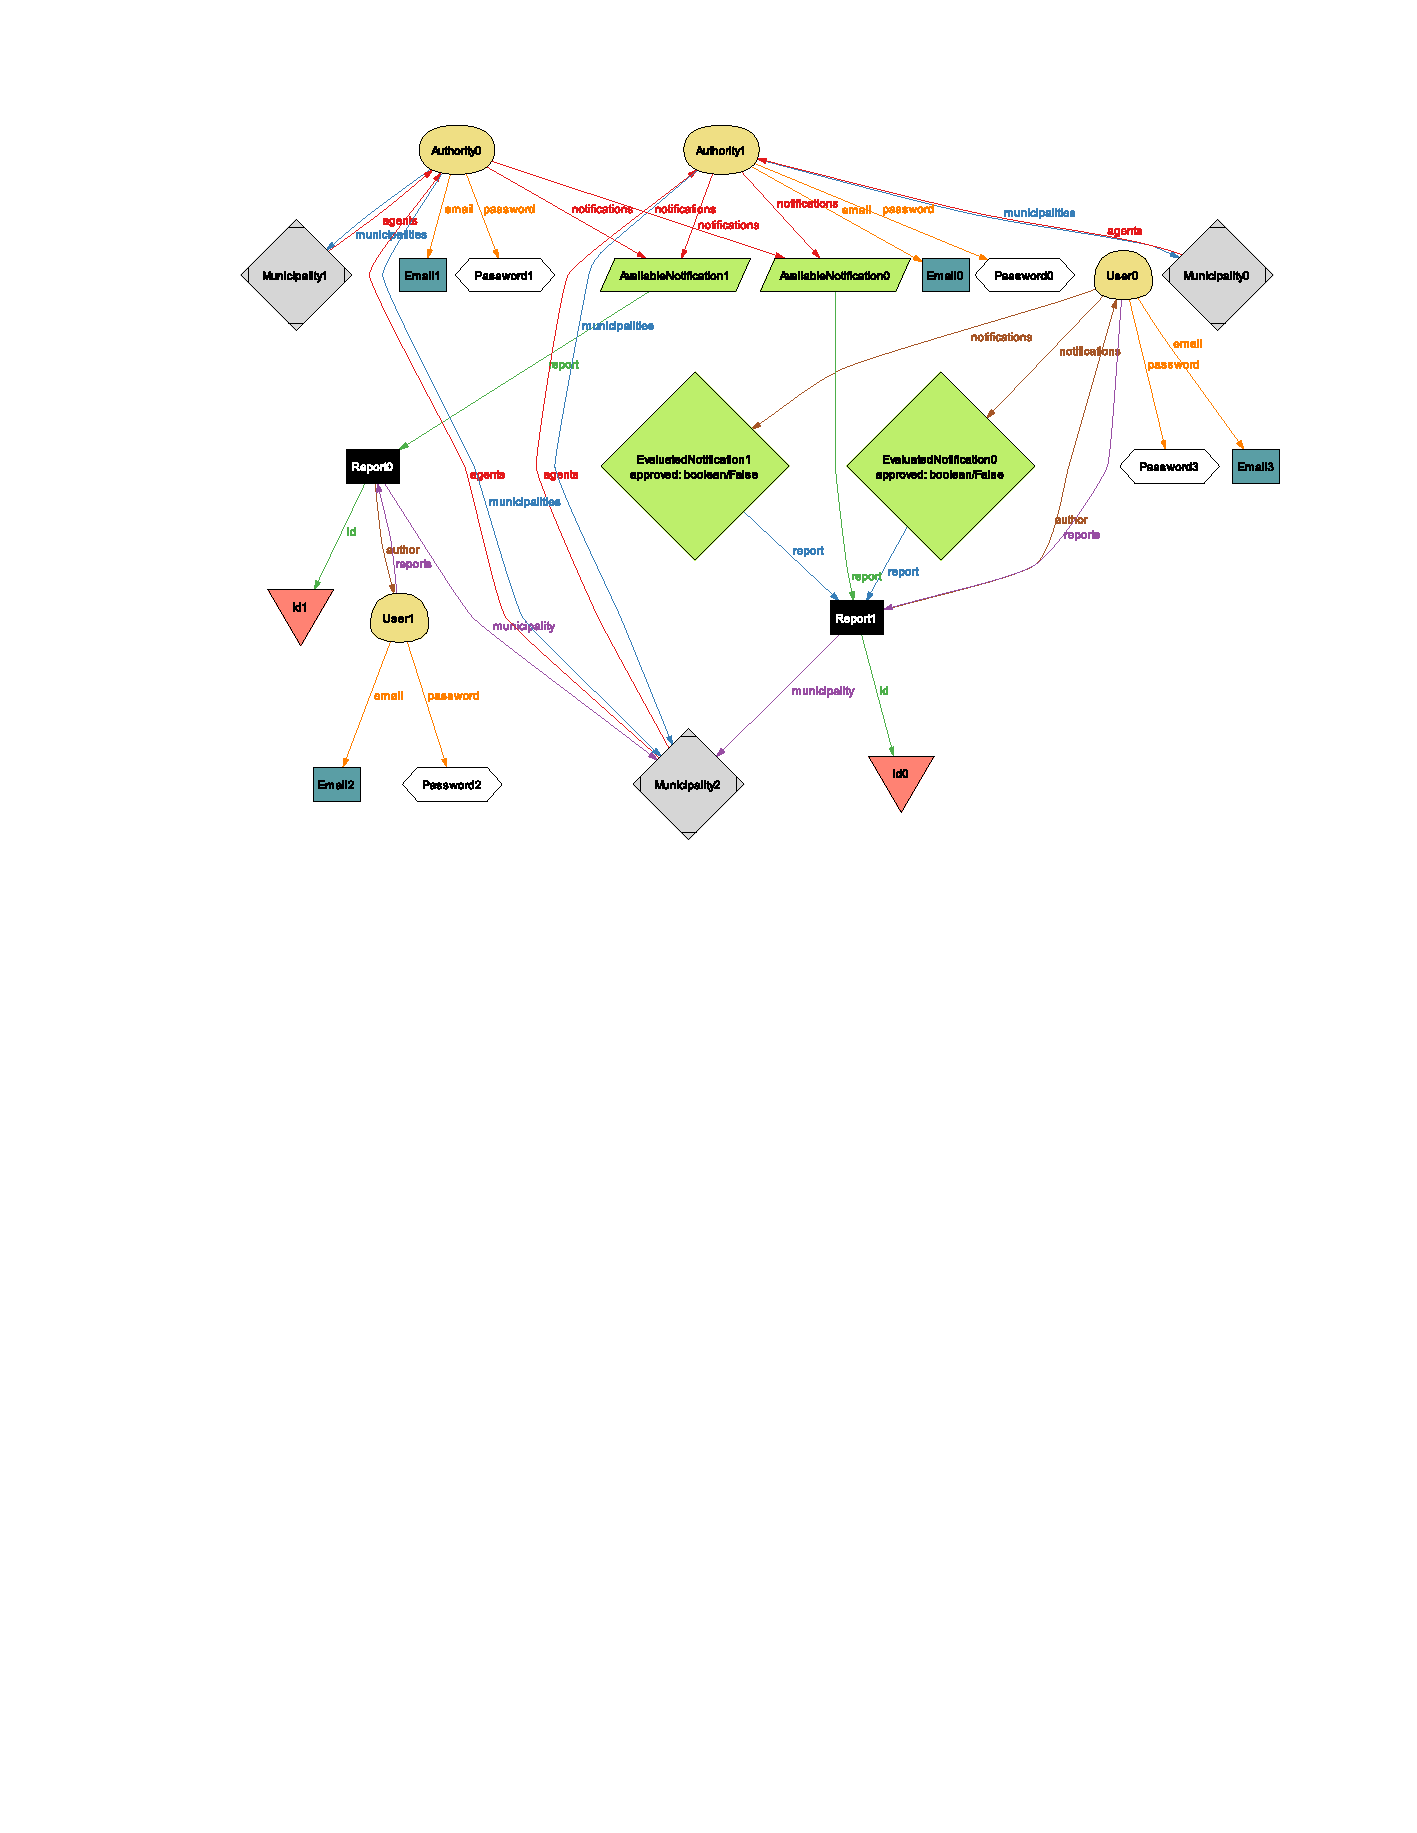
\includegraphics[scale = 1, center]{world1}
		\end{figure}
% End of fourth chapter

\chapter{Effort Spent}
%End of fifth chapter

\chapter{References}
% End of sixth chapter

\end{document}